\documentclass[12pt,a4paper]{report}
\usepackage[left=2.5cm,right=2.5cm,top=3cm,bottom=3cm]{geometry}
\usepackage{fancyhdr}
\usepackage{etoolbox}
\usepackage{titlesec}
\usepackage{titling} % para personalizar el título
\usepackage{amssymb}
\usepackage{amsmath}
\usepackage{graphicx}
\usepackage{ulem}
\usepackage{cancel}
\usepackage{enumitem}
\usepackage{lmodern}
\usepackage{tikz}

\allowdisplaybreaks
\def\arraystretch{1.5}% 

\pagestyle{fancy}
\fancyhf{} 
\fancyhead[L]{UTN-FRC}
\fancyhead[C]{ASyS}
\fancyhead[R]{2R3}
\renewcommand{\headrulewidth}{0.4pt}
\fancyfoot[C]{\vfill\thepage}

\patchcmd{\chapter}{\thispagestyle{plain}}{\thispagestyle{fancy}}{}{}

\renewcommand{\chaptername}{Ejercicio}

\usetikzlibrary{calc, arrows.meta, positioning}

\titleformat{\chapter}[display]
  {\normalfont\bfseries}{\chaptertitlename\ \thechapter}{15pt}{}
\titlespacing*{\chapter}{0pt}{-30pt}{-30pt}

\setlength{\headheight}{15pt}

\DeclareMathSizes{17}{15}{10}{10}

\setlength{\parskip}{6pt}

\title{%
  \fontsize{25}{0}\selectfont Universidad Tecnológica Nacional \\
  \fontsize{22}{30}\selectfont Analisis de Señales y Sistemas \\
  \fontsize{20}{25}\selectfont Trabajo Practico 2
}
\author{
Alejo Agustin Lopez Demichelis\\
Franco Palombo\\
Ignacio Gil\\
Jesus Agustin Frigerio\\
Laureano Valentin Reinoso\\
Luciano Tomas Cortesini Perez\\
Matias Gabriel Moran\\
Leonardo Ramos\\
}
\date{19 / 08 / 2024}

\begin{document}
\maketitle

\chapter{}%ejercicio 1

\textbf{Movimiento Rectilíneo Uniformemente Variado (MRUV) - Caída libre}

\begin{itemize}[left=0pt]
  \item Un primer cuerpo de masa $m_1$ se deja caer (verticalmente) desde una posición inicial $y_0 > 0$.

  \item Un segundo cuerpo de igual masa que el primero, se deja caer (verticalmente) desde una posición inicial 
     $\frac{1}{2} y_0$, es decir, a mitad de camino del primer cuerpo.

\end{itemize}

Teniendo como punto de referencia el "suelo", responder las siguientes consignas:

\begin{enumerate}[label=\alph*),left=0pt]
  \item Realizar un gráfico que represente la situación de los dos cuerpos en caída libre, sus respectivos vectores 
    de velocidad y posición.

  \item Determinar las ecuaciones de cinemáticas para la posición $y_1(t)$ y $y_2(t)$ en función del tiempo para cada
    uno de los cuerpos, respectivamente. \textbf{Reflexionar:} ¿las funciones $y_1, y_2$ pueden interpretarse como 
    señales de variable de tiempo continuo? ¿Las masas de los cuerpos intervienen en la descripción de las funciones
    $y_1(t),y_2(t)$?

    Partimos primero de la ecuacion que determina la posicion de un cuerpo con aceleracion uniforme:
    $$Y(t) = Y_0 + V_0 t + \frac{1}{2} g t^2$$
    Para ambos casos asumimos la velocidad inicial $V_0 = 0$, despreciamos la resistencia del aire y tomamos como valor
    de aceleracion de la gravedad $g = 9.8 \frac{m}{s^2}$:
    $$y_1(t) = Y_0 - \frac{1}{2}9,8\frac{m}{s^2}t^2$$
    $$y_2(t) = \frac{Y_0}{2} - \frac{1}{2}9,8\frac{m}{s^2}t^2$$

    Como se puede observar, las masas no aparecen en las ecuaciones de $y_1(t)$ y $y_2(t)$, por lo que se deduce que las
    masas no intervienen en la descripcion de las funciones.

  \item Calcular el tiempo de vuelo (total) $T$ del primer cuerpo, en función de $y_0$. Similarmente, calcular el
    tiempo de vuelo $\tau$ del segundo cuerpo. ¿Qué relación aritmética encuentra entre los dos tiempos $T$ y $\tau$?
    ¿Se puede obtener $y_2$ como un escalonado en el tiempo de la señal $y_1$?

    Se obtienen los tiempos $T$ y $\tau$ como:
    $$T = \sqrt{\frac{2h}{g}}$$
    $$\tau = \sqrt{\frac{h}{g}}$$
    La relacion aritmetica entonces:
    $$\frac{T}{\tau} = \frac{\sqrt{2}\sqrt{gh}}{\sqrt{gh}}$$
    $$T = \sqrt{2}\tau$$

    No se puede obtener $y_2(t)$ como un escalonado de tiempo de $y_1(t)$. Al escalar el tiempo de $y_1(t)$ por un
    factor de $\sqrt{2}$ queda $y_1(t) = Y_0 - \frac{1}{2}g(\sqrt{2}t)^2$. T y $\tau$ coinciden, es decir los tiempo
    finales son iguales, pero no coinciden las funciones de posicion. Es importante notar que, aunque existe esta
    relacion entre los tiempos de vuelo, no es fisicamente correcto interpretar la posicion $y_2(t)$ del segundo cuerpo
    como una version escalada temporalmente de $y_1(t)$. Los dos cuerpos tienen trayectorias y tiempos de vuelo
    diferentes debido a sus diferentes alturas iniciales, y cada uno debe ser tratado de manera independiente.


  \item Calcular el tiempo $t_0$ que le toma al primer cuerpo estar en la posición $\frac{1}{2} y_0$. ¿Qué relación 
    aritmética encuentra entre $t_0$ y $\tau$? ¿Se puede obtener $y_2$ como una traslación temporal de la señal $y_1$?

    $$\frac{y_0}{2} = Y_0 - \frac{1}{2}g{t_0}^2$$
    $$(\frac{y_0}{2} - Y_0) \cdot (\frac{-2}{g}) = {t_0}^2$$
    $$-\frac{y_0}{2} \cdot (\frac{-2}{g}) = {t_0}^2$$
    $$\sqrt{\frac{y_0}{g}} = t_0$$
    $$t_0 = t$$

    No se puede obtener $y_2(t)$ como una traslacion temporal de $y_1(t)$, porque al desplazar temporalmente $y_1(t)$,
    este no coincide con $y_2(t)$, sin embargo para el $t_0 = t$ si coinciden las posiciones.

  \item \textbf{Reflexionar:} ¿Tiene sentido físico evaluar la señal $y_1$ en tiempos $t > T$? Similarmente, ¿tiene 
    sentido físico evaluar la señal $y_2$ en tiempos $t > \tau$? En caso afirmativo, ¿cuál es la interpretación
    física? Y en caso negativo, emplear alguna herramienta para redefinir las señales $y_1, y_2$, de tal forma que la 
    información provista por el futuro sea nula. Por otra parte, ¿tiene sentido físico evaluar a las señales $y_1,
    y_2$ en tiempos negativos $t < 0$? En caso afirmativo, ¿qué representa? Y en caso negativo, emplear alguna 
    herramienta para redefinir las señales $y_1, y_2$ de tal forma que la información provista por el pasado sea nula.

    No tiene sentido físico evaluar las señales $y_1(t)$ ni $y_2(t)$ en tiempos mayores a T y $\tau$ respectivamente. A
    su vez tampoco tiene sentido evaluar las señales en tiempos negativos, menores a cero. Podríamos definir las señales
    como:
    $$y_1(t) = (Y_0 + V_0t - \frac{1}{2}gt^2)u(t)u(T - t)$$
    $$y_2(t) = (\frac{Y_0}{2} + V_0t - \frac{1}{2}gt^2)u(t)u(\tau - t)$$

  \item Teniendo en cuenta las señales redefinidas del inciso anterior $y_1, y_2$ (pasado y futuro de la señal son
    nulos) verificar si estas cumplen (o no) cada una de las siguientes propiedades: Periódica, Energía finita,
    Potencia finita, causal, acotada.

\begin{enumerate}[label=\alph*)]
    \item Periodicidad

    Las señales $y_1(t)$ y $y_2(t)$ no son periódicas, ya que representan la posición de los cuerpos en caída libre y
    no se repiten en intervalos regulares de tiempo. Cada cuerpo cae una vez y llega al suelo, después de lo cual la
    señal es nula.
    \item Energia

    Las señales $y_1(t)$ e $y_2(t)$ tienen una duración finita en el tiempo (desde t = 0 hasta t = T para $y_1(t)$ y
    hasta t = $\tau$ para $y_2(t)$), y son nulas fuera de estos intervalos, por lo tanto su energía es finita.
    \item Potencia

    Dado que las señales $y_1(t)$ e $y_2(t)$ tienen energía finita, se puede afirmar que tienen una potencia media igual
    a cero.
    \item Causaludad

    Ambas señales son causales por el hecho de estar multiplicadas por los escalones unitarios (u(t)u(T - t) para
    $y_1(t)$ y  u(t)u($\tau$ - t) para $y_2(t)$) que anulan el pasado y futuro de las mismas.
    \item Modulo

    Las señales $y_1(t)$ e $y_2(t)$ son acotadas en sus respectivos intervalos de tiempo. Para $y_1(t)$ la máxima
    magnitud ocurre en t = 0 y es $Y_0$. Para $y_2(t)$ la máxima magnitud también ocurre en t = 0  y es
    $\frac{1}{2}Y_0$.
\end{enumerate}

\end{enumerate}

\textbf{Movimiento Armónico Simple (MAS) - Masa/Resorte}

Considerar un sistema conformado por una Masa $m$, atada a la derecha de un resorte con constante elástica $\kappa$, 
dispuesto en forma horizontal y sujetado en el extremo izquierdo. Teniendo como punto de referencia la posición de
equilibrio, máxima amplitud $A > 0$ y despreciando los efectos de la fricción, responde las siguientes consignas:

\begin{enumerate}[label=\alph*),left=0pt]
  \item Realizar un gráfico que represente el sistema y sus respectivos vectores de fuerza.

  \item Determinar la ecuación de cinemática para la posición $x(t)$ en función del tiempo. \textbf{Reflexionar:} ¿la
    función $x$ puede interpretarse como una señal de variable de tiempo continua?

    Partiendo de la ecuacion diferencial de un oscilador armonico simple $m \frac{dt^2}{d^2x} + kx = 0$, determinamos
    la ecuacion de cinematica para la posicion en funcion del tiempo $x(t) = A \sin(\omega t + \phi)$. Si, la funcion
    $x(t)$ puede interpretarse como una señal de variable de tiempo continuo.

  \item Es de conocimiento general que la función posición $x(t)$ se puede determinar en función del $seno$ o del
    coseno. Determinar la transformación temporal sobre la señal, la cual permite pasar de la formulación $seno$ a la
    formulación $coseno$.

    Para pasar de la formulación seno a la formulación coseno debe aplicarse una traslación temporal a la señal
    correspondiente al desfase entre las funciones trigonométricas seno y coseno, es decir sumar $\frac{\pi}{2}$.
    Entonces:

    $$A \sin(\omega t + \frac{\pi}{2}) = A \cos(\omega t)$$

  \item Verificar si la señal $x(t)$ cumple (o no) cada una de las siguientes propiedades: Periódica, Energía finita,
    Potencia finita, causal, acotada.

  \begin{enumerate}[label=\alph*)]
    \item Periodica

      Es periodica ya que existe un valor T tal que $x(t) = x (t + nT)$, donde n = 1,2,3..
    \item Energia

    Tiene energia infinita. Para señales periodicas, la energia total en el sentido clasico puede ser infinita debido a
    que la señal se repite indefinidamente, pero si hablamos de la energia en un periodo T, es finita y es:

    $$E_T = \int_{0}^{T} |A \cos(\omega t)|^2 dt$$
    $$E_T = A^2 \int_{0}^{T} \cos(\omega t)^2 dt$$
    $$E_T = A^2 \int_{0}^{T} \frac{1 + \cos(2 \omega t)}{2} dt$$
    $$E_T = A^2 \frac{1}{2}\int_{0}^{T}  \cos(2 \omega t)dt$$
    \item Potencia

    Tiene energia infinita si consideramos el intervalo $(-\infty,\infty$, pero la energia es finita en un solo periodo,
    por lo que la potencia media es finita:

    $$P_{med} = \lim_{T \to \infty} \frac{1}{2T} E_T$$
    $$P_{med} = \lim_{T \to \infty} \frac{A^2T}{4T} = \frac{A^2}{4}$$
    $$P_T = 2 P_{med} = \frac{A^2}{2}$$
    \item Acotada

    La señal es acotada ya que para todo t, $x(t) <= A$ siendo A la amplitud. Esto se da ya que las funciones
    trigonometricas seno o coseno toman valores entre -1 y 1
    \item Causal

    La señal no es causal porque esta definida para todos los tiempos, $t \in (-\infty,\infty)$
  \end{enumerate}
\end{enumerate}

\chapter{}%ejercicio 2
Considerar las siguientes señales proporcionadas por un rectificador de onda completa y $1/2$ onda respectivamente:

\textbf{Señal Sinusoidal rectificada de onda completa}, $x_1(t)$ determinada por el gráfico:
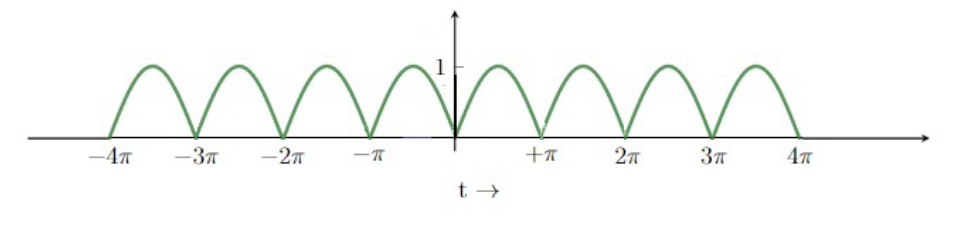
\includegraphics[width=\textwidth]{images/ej2.a.png}

\textbf{Señal Sinusoidal rectificada de media onda}, $x_2(t)$ determinada por el gráfico:
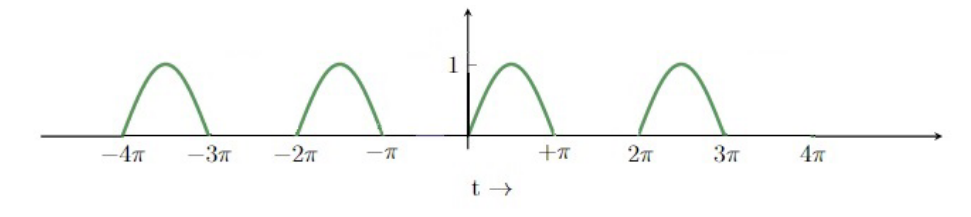
\includegraphics[width=\textwidth]{images/ej2.b.png}

\begin{enumerate}[label=\alph*),left=0pt]
  \item Calcular el periodo fundamental $T_0$ de las señales $x_1, x_2$. ¿Las señales tienen energía finita? Calcular
    la energía relativa a un intervalo con longitud un periodo fundamental $T_0$.\\
    \textbf{Señal sinusoidal rectificada de media onda}

    Esta señal tiene la siguiente representación analítica:
    $$x(t)=
    \begin{cases}
      sen(t), & 0<t<\pi\\
      0, & \pi<t<2\pi
    \end{cases}
    $$

    $$
    \begin{aligned}
      E &= \int_{0}^{\pi} |\sin(t)|^2 \, dt \\
        &= \int_{0}^{\pi} \sin^2(t) \, dt
    \end{aligned}
    $$

    $$
    \text{utilizando la siguiente identidad: }
    \sin^2(t) = \frac{1 - \cos(2t)}{2}
    $$

    $$
    \begin{aligned}
      E &= \int_{0}^{\pi} \frac{1 - \cos(2t)}{2} \, dt \\
        &= \frac{1}{2} \left( \int_{0}^{\pi} 1 dt - \int_{0}^{\pi} \cos(2t) \, dt \right)
    \end{aligned}
    $$

    \text{Resolviendo la integral por sustitución}

    $$u = 2t, \quad du = 2dt \quad \Rightarrow \quad dt = \frac{du}{2}$$

    $$
    \begin{aligned}
       E &= \frac{1}{2} \left( \pi - \frac{1}{2} \int_{0}^{2\pi} \cos(u) \, du \right) \\
         &= \frac{\pi}{2} - \frac{1}{4} \left( \sin(2\pi) - \sin(0) \right) \\
         &= \frac{\pi}{2}
    \end{aligned}
    $$

    \textbf{Energía en el período:}
    $$T_0 = \pi$$

    El período fundamental $T_0>0$, se determina por:

    $$
      \begin{aligned}
      x(t) &= x(t+T_0)\\
      sen(t)&=sen(t+T_0) \Rightarrow T_0=2\pi
      \end{aligned}
    $$

    Las señales son periódicas y por lo tanto tienen energía infinita. 

    Energía relativa a un periódo $T_0$:
    $$
    \begin{aligned}
      E_{T_{0}}&=\int_0^{2\pi}|x(t)|^2=\int _0^\pi sen(t)^2dt=\int_0^\pi \frac{1}{2}(1-cos(2t) dt\\
            E_{T_0}&=\frac{t|^\pi_0}{2}-\frac{sen(2t)|^\pi_0}{2}\\
      E_{T_0}&=\frac{\pi}{2}
    \end{aligned}
    $$

  \item Teniendo en cuenta que la potencia media de una señal se define como

    $$P_1 = \lim_{r \to \infty} \frac{1}{2r} \int_{-r}^{r} |x(t)|^2 \, dt$$

    \begin{itemize}[left=0pt]
      \item Demostrar la siguiente igualdad, válida para señales periódicas en donde la potencia media relativa a un
        intervalo con longitud un periodo fundamental $T_0$ coincide con la potencia media, es decir:

         $$P_1 = \frac{1}{T_0} \int_{t_0}^{t_0 + T_0} |x(t)|^2 \, dt$$

        \textbf{Demostración}

        Sea la potencia media definida como:

        $$P_m=\lim _{r \to \infty} \frac{1}{2r}\int_{-r}^{r}|x(t)|^2dtk$$

        Si x(t) es periódica con período T, entonces el integrando de la potencia media es igual
        para cualquier intervalo de longitud T, permitiendo que el límite se tome de manera tal 
        que 2L sea un múltiplo entero del período  $2T=mr$, la energía total de x(t) sobre un intervalo de longitud $2r$ is m veces la energía sobre un período. Por lo tanto la potencia media es:

        $$P_m=\lim_{r to \infty}[\frac{1}{mT}m\int_{t_0}^{t_0+T} |x(t)|^2 dt]=\frac{1}{T}\int_{t_0}^{t_0+T} |x(t)|^2 dt$$

      \item Calcular la potencia media $P_1$ de la señal $x_1$ y similarmente, $P_2$ de la señal $x_2$\\
        La potencia media para la señal 2 es:

        $$
        \begin{aligned}
        P_{2m}&=\frac{1}{2\pi}\int_0^{\pi}|sen(t)|^2dt
        =\frac{1}{2\pi}\int_0^{\pi}sen(t)^2dt\\
        &=\frac{1}{2\pi}\int_0^{\pi}\frac{1}{2}(1-\cos (2t))dt
        =\frac{1}{4\pi}\{t\vert_0^\pi-\frac{1}{2}senz(2t)\vert_0^\pi\}\\
        &=\frac{1}{4\pi}[\pi-0+1-1]\\
        P_{2m}&=\frac{\pi}{4\pi}
        =\frac{1}{4}
        \end{aligned}
        $$

    \end{itemize}

    $$ P = \frac{1}{T_0} \int_{t_0}^{t_0 + T_0} |x(t)|^2 \, dt $$

    \textbf{Donde}

    $$
    \begin{aligned}
      t_0 &= 0 \quad \text{y} \quad T_0 = \pi \\
      \Longrightarrow P &= \frac{1}{\pi} \int_{0}^{\pi} |\sin(t)|^2 \, dt \\
      &= \frac{1}{\pi} \int_{0}^{\pi} \sin^2(t) \, dt
    \end{aligned}
    $$

    \textbf{Como}

    $$
    \sin^2(t) = \frac{1 - \cos(2t)}{2}
    $$

    \text{Resuelvo integrando por sustitución}

    $$
    \begin{aligned}
      u &= 2t, \quad du = 2 \, dt \quad \Longrightarrow \quad dt = \frac{du}{2}
    \end{aligned}
    $$

    $$ P = \frac{1}{2\pi} \left( \int_{0}^{\pi} dt - \frac{1}{2} \int_{0}^{2\pi} \cos(u) \, du \right) $$

    Resolvemos las integrales:

    $$
    \begin{aligned}
      P &= \frac{1}{2\pi} \left( \pi - \frac{1}{2} \left( \sin(2\pi) - \sin(0) \right) \right) \\
         &= \frac{1}{2\pi} \left( \pi - 0 \right) \\
         &= \frac{1}{2\pi} \times \pi \\
         &= \frac{1}{2}
    \end{aligned}
    $$

  \item Considerar el conjunto de señales básicas

    $$\{\psi_n(t) = \cos(n\omega t) \mid n \geq 0\} \cup \{\varphi_n(t) = \sin(n\omega t) \mid n \geq 1\}$$

      \begin{itemize}[left=0pt]
      \item Calcular la energía relativa a un intervalo con longitud un periodo fundamental $T_0$ y el periodo $T_n$
        de cada señal del conjunto, y luego, demostrar que (dos a dos) forman un conjunto de señales ortogonales más no
        ortonormales.
    $$
    \begin{aligned}	
    E_{T_0}&=\int^{\frac{2\pi}{\omega_0}}_0 sen^2(nw_0t)dt
    \\
    &=\int^{\frac{2\pi}{\omega_0}}_0\frac{1}{2}(1-cos(2nw_0t)dt\\
    E_{T_0}&=\frac{t|^{\frac{2\pi}{\omega_0}}_0}{2}-\frac{cos(2n\omega_0t)|^{\frac{2\pi}{\omega_0}}_0}{2n\omega_0}\hspace{1cm}(1)
    \end{aligned}
    $$

    Para todo n la segunda parte de la ecuación es 0, ya que es una función coseno que se integra en $2n$ periódos, lo cual da 0. Por lo tanto:

    $$ E_{T_0}=\frac{\pi}{\omega_0} $$

    En el caso de calcular la energía relativa a $T_n$, lo único que cambia son los límtes 
    de integración, de todos modos la segunda parte de la ecuación sigue siendo 0, ya que se 
    integra una función coseno en 2 períodos. y la energía relativa a $T_n$ es por lo tanto:

    $$ E_{T_n}=\frac{t|^{\frac{2n\pi}{\omega_0}}_0}{2}=\frac{2n\pi}{2\omega_0}=\frac{n\pi}{\omega_0} $$

        Se dice que un conjunto de señales es ortogonal sobre un intervalo $(a,b)$ si:

    $$
    I=\int^b_a\phi_l(t)\phi^*_kdt=\begin{cases}
        E_k,& l=k\\
        0, & l\neq k
    \end{cases}
    $$

    Se dice que es ortonormal en el caso en que $E_k=1$.

    En nuestro caso sobre un intervalo $T_0=\frac{2\pi}{\omega_0}$, debemos calcular si el conjunto es ortogonal.

    $$ E_{T_0}=\int_0^{T_0}sen(n\omega_0t)sen(m\omega_0t)dt $$

    $$ =\frac{1}{2}\int_0^{T_0}[cos((m-n)\omega_0 t)-cos((m+n)\omega_0 t)]dt $$

    En el caso en que $m=n$ estamos en el mismo caso que en (1) del inciso anterior, por lo tanto 

    $$
    I=\frac{\pi}{\omega_0}, \hspace{1cm}n=m
    $$

    En el caso en que $m\neq n$:
    $$
    I=\frac{1}{2}(\frac{sen((m-n)\omega_0t)}{(m-n)\omega_0}-\frac{sen((m+n)\omega_0t)}{(m+n)\omega_0})|^{t_0+T_0}_{t_0}
    $$

    Tanto $m-n$ como $m+n$ son números enteros, por lo tanto se integra un número entero de veces sobre un período, es decir que ambas integrales valuadas dan 0. Por lo tanto:
    $$
    I=\begin{cases}
        \frac{\pi}{\omega_0},&n=m\\
        0,&\forall n\neq m
    \end{cases}
    $$
    No son ortonormales porque $\frac{\pi}{\omega_0}\neq 0$	


	\textbf{Reflexión:} ¿si los periodos $T_n$ de cada señal del conjunto básico son distintos, por qué la suma 
      (finita/infinita) es periódica? \\
	Porque el periodo $T_0$ es n veces el periodo de la señal enésima, por lo tanto todas comparten el periodo $T_0$, por lo tanto su suma finita/infinita es periódica de periodo $T_0$.\\

	¿Por qué se restringe el dominio del tiempo en un intervalo del tipo 
      $t_0 \leq t \leq t_0 + T_0$, si las señales básicas están bien definidas en todo el eje temporal?\\
		Porque si definimos la señal en todo el eje temporal, la energía de dicha señal es infinita.
   \item Obtener la representación de las señales $x_1, x_2$ como una combinación lineal de las señales básicas, 
     esto es, calcular coeficientes $(a_n, b_n)$ en $\mathbb{R}$ tales que:

     $$x_1 = \sum_{n=0}^{\infty} a_n \psi_n + \sum_{n=1}^{\infty} b_n \varphi_n$$
     Similarmente para la señal $x_2$.\\

  \textbf{Señal $x_1$}\\
  Para calcular los coeficientes \(a_n\) y \(b_n\) de la serie de Fourier, seguimos los siguientes pasos:

  $$
  \begin{aligned}
    a_0 &= \frac{1}{\pi} \int_0^\pi |\sin(t)| \, dt \\
        &= \frac{1}{\pi} \int_0^\pi \sin(t) \, dt \\
        &= \frac{1}{\pi} \left[ -\cos(t) \right]_0^\pi \\
        &= \frac{1}{\pi} \left[ -\cos(\pi) - (-\cos(0)) \right] \\
        &= \frac{1}{\pi} \left[ -(-1) - (-1) \right] \\
        &= \frac{1}{\pi} \left[ 1 + 1 \right] \\
        &= \frac{2}{\pi}
  \end{aligned}
  $$
  
  Ahora calculamos \(a_n\):
  
  $$
  \begin{aligned}
    a_n &= \frac{2}{\pi} \int_0^\pi \sin(t) \cos(2nt) \, dt \\
        &= \frac{1}{\pi} \int_0^\pi 2 \sin(t) \cos(2nt) \, dt \\
        &= \frac{1}{\pi} \int_0^\pi \left[ \sin(t + 2nt) + \sin(t - 2nt) \right] \, dt \\
        &= \frac{1}{\pi} \left[ \int_0^\pi \sin(t(1 + 2n)) \, dt + \int_0^\pi \sin(t(1 - 2n)) \, dt \right]
  \end{aligned}
  $$
  
  Integrando por sustitución:
  
  $$
  \begin{aligned}
    u &= t(1 + 2n) \quad \text{entonces} \quad du = (1 + 2n) \, dt \quad \Longrightarrow \quad dt = \frac{du}{1 + 2n} \\
    v &= t(1 - 2n) \quad \text{entonces} \quad dv = (1 - 2n) \, dt \quad \Longrightarrow \quad dt = \frac{dv}{1 - 2n} \\
    &= \frac{1}{\pi} \left[ \int_0^{\pi(1+2n)} \frac{\sin(u)}{1+2n} \, du + \int_0^{\pi(1-2n)} \frac{\sin(v)}{1-2n} \, dv \right] \\
    &= \frac{1}{\pi} \left[ \frac{-\cos(\pi(1+2n)) + \cos(0)}{1+2n} + \frac{-\cos(\pi(1-2n)) + \cos(0)}{1-2n} \right] \\
    &= \frac{1}{\pi} \left[ \frac{-\cos(\pi(1+2n)) + 1}{1+2n} + \frac{-\cos(\pi(1-2n)) + 1}{1-2n} \right]
  \end{aligned}
  $$
  
  
  
  \text{Sabiendo que:}

  $$
  \begin{aligned}
  \cos(\pi(1+2n)) = \cos(\pi + 2n\pi) = -\cos(2n\pi) \\
  \cos(\pi(1-2n)) = \cos(\pi - 2n\pi) = -\cos(2n\pi) \\
  \end{aligned}
  $$

  $$
  \begin{aligned}
    &= \frac{1}{\pi} \left[ \frac{-(-\cos(2n\pi)) + 1}{1+2n} + \frac{-(-\cos(2n\pi)) + 1}{1-2n} \right] \\
    &= \frac{1}{\pi} \left[ \frac{\cos(2n\pi) + 1}{1+2n} + \frac{\cos(2n\pi) + 1}{1-2n} \right] \\
    &= \frac{1}{\pi} \left[ \frac{2\cos(2n\pi) + 2}{1 - 4n^2} \right] \\
    &= \frac{2}{\pi} \left[ \frac{\cos(2n\pi) + 1}{1 - 4n^2} \right] \\
    &= \frac{2}{\pi} \left[ -\frac{\cos(2n\pi) + 1}{4n^2 - 1} \right] \\
    &= -\frac{2}{\pi (4n^2 - 1)} (\cos(2n\pi) + 1)
  \end{aligned}
  $$
  
  Dado que \(\cos(2n\pi) = 1\) para todo \(n \in \mathbb{N}\):
  
  $$
  \begin{aligned}
    a_n &= -\frac{2}{\pi (4n^2 - 1)} (1 + 1) \\
        &= -\frac{4}{\pi (4n^2 - 1)}
  \end{aligned}
  $$
  
  Finalmente, calculamos los coeficientes \(b_n\):
  
  $$
  \begin{aligned}
    b_n &= \frac{1}{\pi} \int_0^\pi \sin(t) \sin(2nt) \, dt \\
        &= \frac{1}{\pi} \int_0^\pi \sin(t) \sin(2nt) \, dt \\
  \end{aligned}
  $$

  $$
  \text{utilizando la siguiente identidad: }
  \sin(A)\sin(B) = \frac{1}{2} (\cos(A - B) - \cos(A + B)) \\
  $$

  $$
  \begin{aligned}
    &= \frac{1}{\pi} \int_0^\pi \frac{1}{2} (\cos(t - 2nt) - \cos(t + 2nt)) \, dt \\
    &= \frac{1}{2\pi} \left[ \int_0^\pi \cos(t - 2nt) \, dt - \int_0^\pi \cos(t + 2nt) \, dt \right]
  \end{aligned}
  $$
  
  Integrando por sustitución:
  
  $$
  \begin{aligned}
    u &= t(1 - 2n) \quad \text{entonces} \quad du = (1 - 2n) \, dt \quad \Longrightarrow \quad dt = \frac{du}{1 - 2n} \\
    v &= t(1 + 2n) \quad \text{entonces} \quad dv = (1 + 2n) \, dt \quad \Longrightarrow \quad dt = \frac{dv}{1 + 2n} \\
    &= \frac{1}{2\pi} \left[ \frac{1}{1 - 2n} \int_0^{\pi(1 - 2n)} \cos(u) \, du - \frac{1}{1 + 2n} \int_0^{\pi(1 + 2n)} \cos(v) \, dv \right] \\
    &= \frac{1}{2\pi} \left[ \frac{1}{1 - 2n} (\sin(\pi (1 - 2n)) - \sin(0)) - \frac{1}{1 + 2n} (\sin(\pi (1 + 2n)) - \sin(0)) \right]
  \end{aligned}
  $$
  
  Dado que \(\sin(\pi (1 - 2n)) = 0\) y \(\sin(\pi (1 + 2n)) = 0\) para todo \(n\):
  
  $$
  \begin{aligned}
    &= \frac{1}{2\pi} \left[ \frac{1}{1 - 2n} \cdot 0 - \frac{1}{1 + 2n} \cdot 0 \right] \\
    &= 0
  \end{aligned}
  $$
  
  Por lo tanto, los coeficientes \(b_n\) son cero para todo \(n\):
  
  $$
  b_n = 0 \quad \forall \, n
  $$
  

	\textbf{Señal $x_2$}\\

Para calcular los coeficientes $a_n$ y $b_n$ podemos hacer uso de los coeficientes $c_n$ de la serie exponencial de la serie de Fourier y luego aplicar el cambio de coordenadas para hallarlos:
            $$
            \begin{aligned}
                c_n &= \frac{1}{T} \int_0^T \sin t \exp\left(-j\frac{2\pi n t}{T}\right) dt\\
                &= \frac{1}{2\pi} \int_0^{\pi} \frac{1}{2j}\left(e^{jt} - e^{-jt}\right) e^{-jnt} dt\\
                &= \frac{1}{4\pi j} \int_0^{\pi} \left(e^{-j(n-1)t} - e^{-j(n+1)t}\right) dt \hspace{1cm}(1)\\
                &= \frac{e^{-jn\pi/2}}{2\pi(1-n^2)} \left(e^{-jn\pi/2} + e^{jn\pi/2}\right)\\
                & = \frac{1}{\pi(1-n^2)} \cos\left(\frac{n\pi}{2}\right)e^{-jn\pi/2}, \quad n \neq \pm 1\\
                c_n &= \begin{cases}
            \frac{1}{\pi(1-n^2)}, & n \text{ even} \\[5pt]
            0, & n \text{ odd}, \quad n \neq \pm 1
            \end{cases}
            \end{aligned}
            $$

       Para el caso en donde n=-1,1, necesitamos evaluar la integral primero y resolver despuésde tal forma utilizando (1), calculamos:

       $$
       \begin{aligned}
       c_1&=\frac{1}{4\pi j}\int_0^\pi(e^{-j(1-1)}-e^{-j(1+1)t})dt\\
       &=\frac{1}{4\pi j}\int^\pi_0 (1-e^{-j2t})dt=\frac{t|^\pi_0}{4\pi j}-\frac{e^{-2jt}|^\pi_0}{4\pi j (-2j)}\\
       c_1&=\frac{\pi}{4\pi j}-0=\frac{1}{4j}=\frac{-j}{4}
       \end{aligned}
       $$
     
       $$
        \begin{aligned}
        c_{-1}&=\frac{1}{4\pi j}\int^\pi_0(e^{-j(-1-1)}-e^{-j(-1+1)t})dt\\
       c_{-1}&=\frac{1}{4\pi j}(0-\pi)=\frac{-1}{4j}=\frac{j}{4}     
        \end{aligned}
       $$

       De esta forma:
       $$
       c_n = \begin{cases}
            \frac{1}{\pi(1-n^2)}, & n \text{ even} \\[5pt]
            0, & n \text{ odd}, \quad n \neq \pm 1 \\
            \frac{j}{4}, & n=-1 \\
            \frac{-j}{4} & n=1
            \end{cases}$$

        Para calcular los coeficientes $a_n$ y $b_n$ simplemente debemos conocer la matriz de cambio de base la cual es $a_0=c_0,\hspace{0.3cm}a_n=2Re(C_n)\hspace{0.3cm}b_n=-2Im(C_n)$.
        Por lo tanto:
        $$
        \begin{aligned}
            b_n&=\begin{cases}
            \frac{1}{2},& n=1\\
            0, & \forall n >1
        \end{cases}\\
        a_0&=\frac{1}{\pi}\\
        a_n&=\begin{cases}
            0,&\forall n \hspace{0.1cm}impar\\
            \frac{2}{\pi(1-n^2)},& \forall n \hspace{0.1cm} par
        \end{cases}\\  
        \end{aligned}
        $$
        Entonces podemos representar a $x(t)$ como:
        $$
        x(t)=\frac{1}{\pi}+\frac{1}{2}sen(t)+\frac{2}{\pi}[\frac{1}{1-4}cos(2t)+\frac{1}{1-16}cos(4t)+\dots]
        $$


   \item Truncar la suma infinita del inciso anterior en $n = 5$ y hacer un gráfico comparativo entre la señal 
     original $x_1$ y su aproximación trigonométrica. Similarmente para la señal $x_2$.\\

\textbf{Señal $x_1$}\\
     Finalmente, truncamos la serie hasta \(n = 5\) y obtenemos los siguientes coeficientes \(a_n\):
  
     $$
     \begin{aligned}
       a_0 &= \frac{2}{\pi} \\
       a_1 &= \frac{4}{3\pi} \\
       a_2 &= \frac{4}{15\pi} \\
       a_3 &= \frac{4}{35\pi} \\
       a_4 &= \frac{4}{63\pi} \\
       a_5 &= \frac{4}{99\pi}
     \end{aligned}
     $$

\textbf{Señal $x_2$}\\

Si truncamos la suma en $n=5$ entonces podemos aproximar a la señal como:
        $$
        x(t)=\frac{1}{\pi}+\frac{1}{2}sen(t)+\frac{2}{\pi}[\frac{1}{1-4}cos(2t)+\frac{1}{1-16}cos(4t)]
        $$
 El gráfico de dicha señal comparada con la original es:\\

%grafico aprox senal 2
\textbf{Señal $x_2$}\\

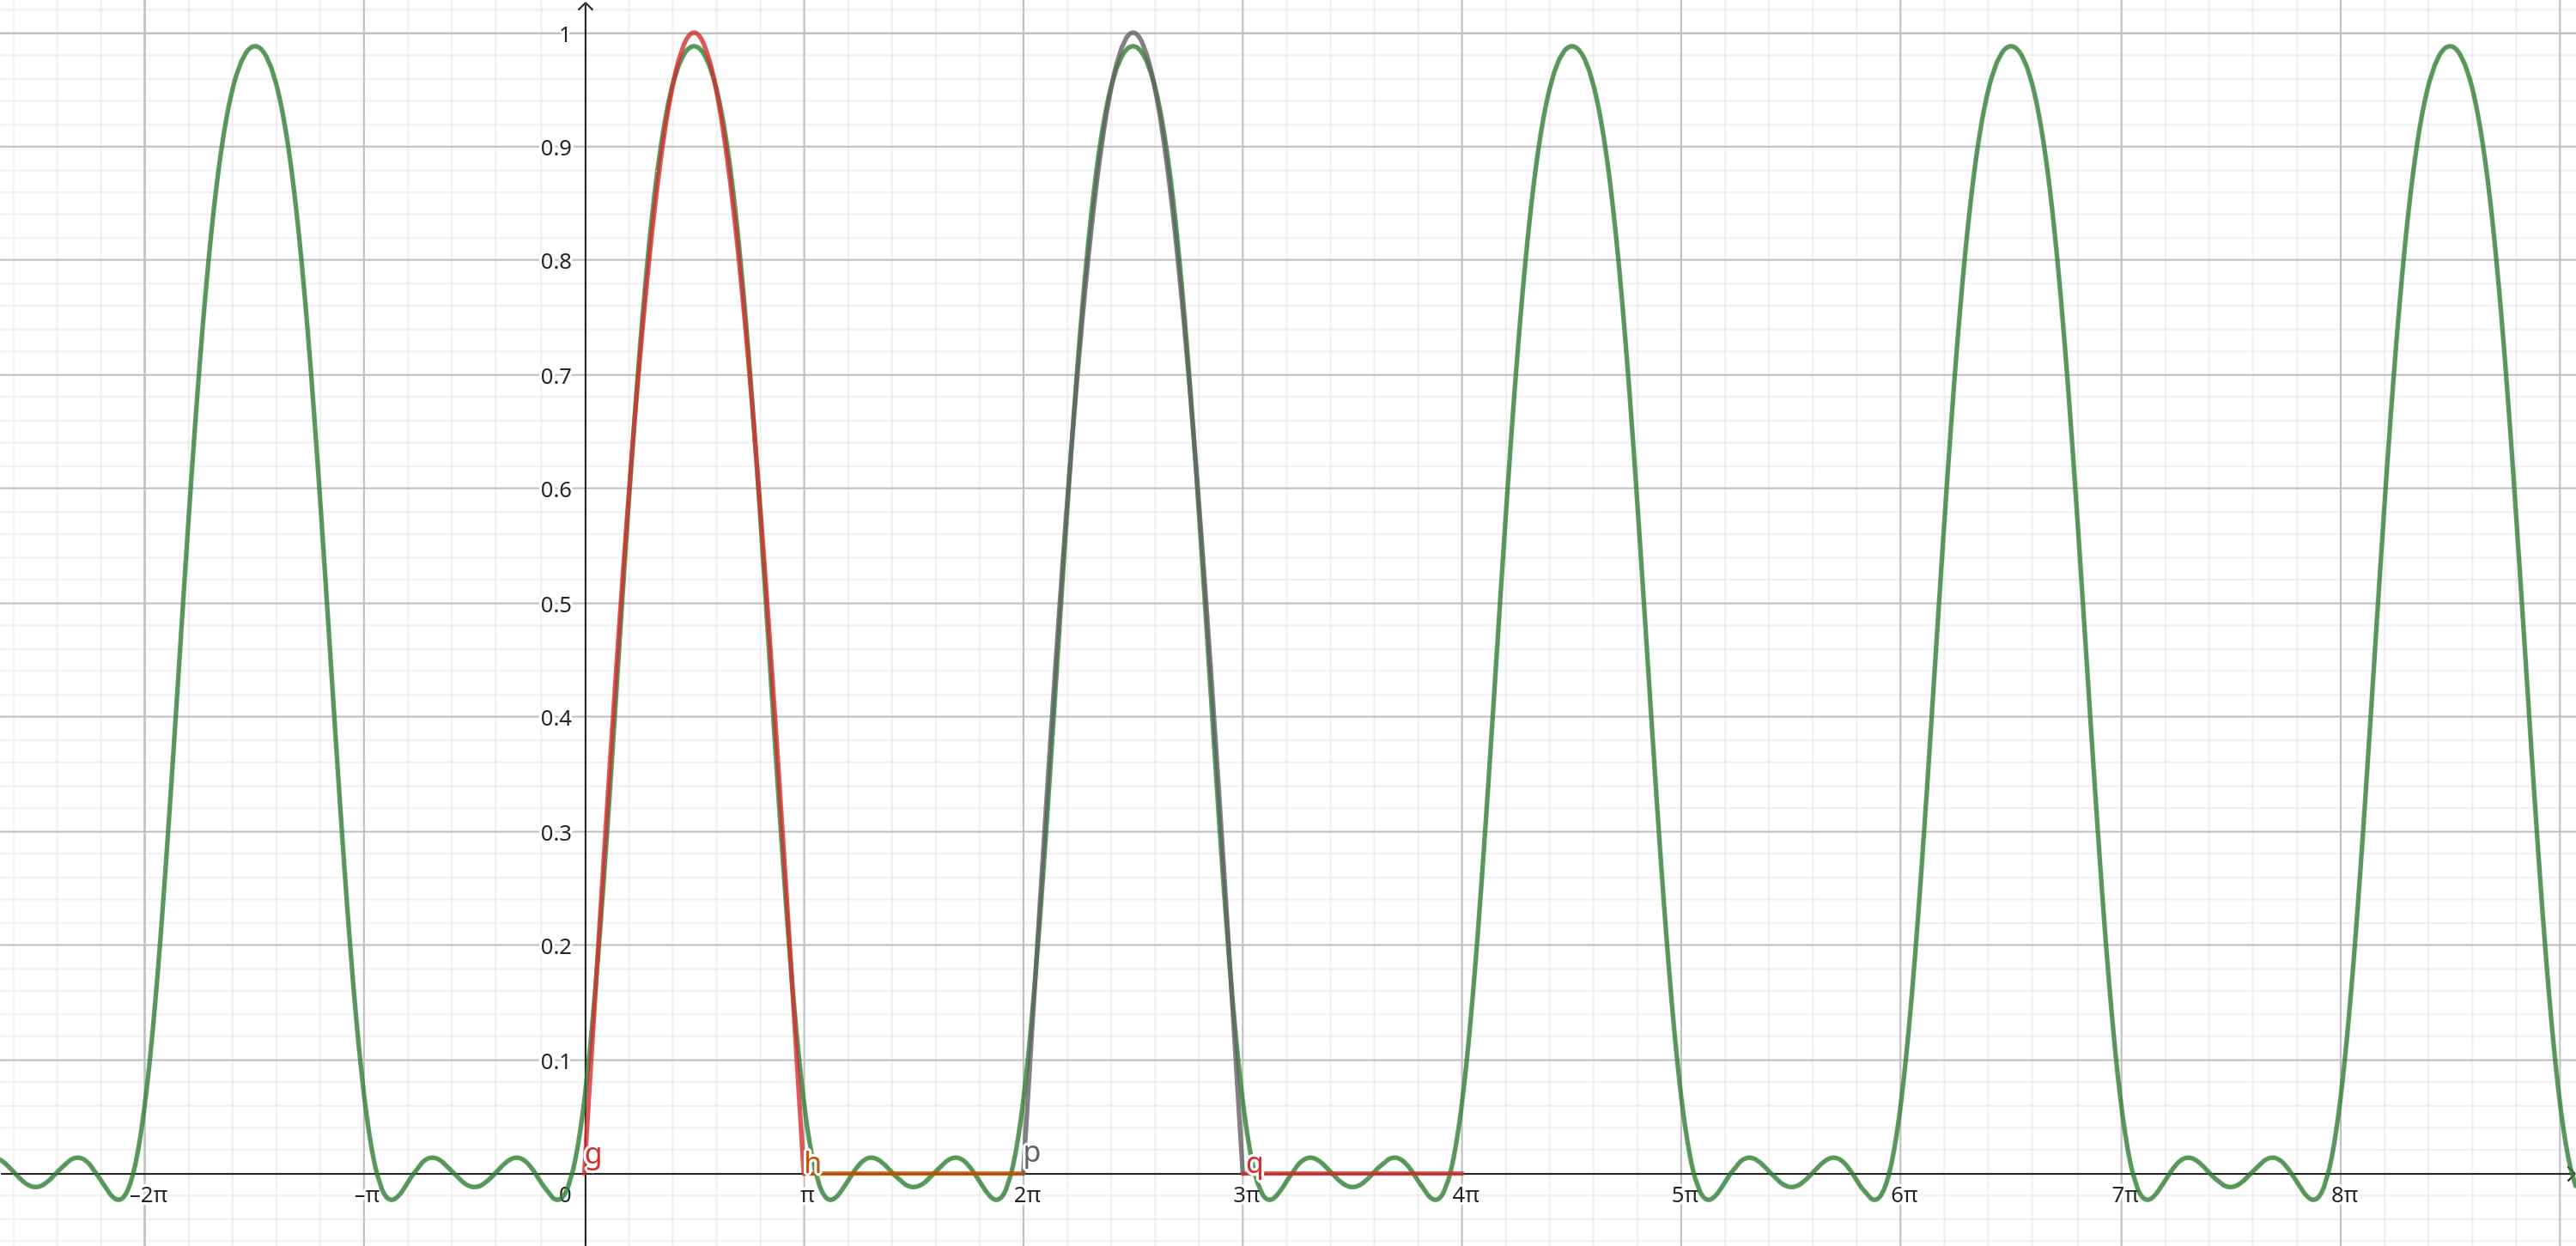
\includegraphics[width=0.9\textwidth]{images/ej2.2a.png}

  \end{itemize}

  \item Considerar el conjunto de señales básicas

  $$\{\phi_n(t) = e^{jn\omega t} \mid n \in \mathbb{Z}\}$$

  Notar que la siguiente relación entre las señales con parámetro negativo y el conjugado:

  $$\phi(-n) = \phi_n^*, \forall n \geq 0$$

  \begin{itemize}[left=0pt]

    \item Calcular la energía relativa a un intervalo con longitud un periodo fundamental $T_0$ y el periodo $T_n$ de
      cada señal del conjunto, y luego, demostrar que (dos a dos) forman un conjunto de señales ortogonales más no
      ortonormales.\\

	Energía relativa a $T_0$:
	$$
	E_{T_0}=\int_0^{\frac{2\pi}{\omega_0}}e^{jnwt}e^{-jnwt}dt=\int_0^{\frac{2\pi}{\omega_0}}e^0dt=\int^{\frac{2\pi}{\omega_0}}_01dt=
		  t|^{\frac{2\pi}{\omega_0}}_0=\frac{2\pi}{\omega_0}
	$$
Energía relativa a $T_n$:
	$$
	    \int^{T_n}_0e^{jn\omega t}e^{-jn\omega t}dt=t|^{T_n}_0=T_n=\frac{2\pi}{\omega_0n}
	$$

\textbf{Demostración ortogonalidad:}
$$
\begin{aligned}
	I&=\int^{T_0}_0e^{jn\omega t}e^{-jm\omega t}dt\\
	&=\int_0^{T_0}e^{j\omega t(n-m)}dt\\
\end{aligned}
$$
	En el caso en que $n=m$ estamos en el mismo caso que cuando calculamos la energía relativa a $T_0$
	, por lo tanto $I=T_0$.\\
	Cuando $n\neq m$ entonces:
		  $$
		  \begin{aligned}
			  I&=\frac{e^{j\omega t(n-m)}}{\omega(n-m)}|^{T_0}_0
			    =\frac{e^{j\omega T_0(n-m)}}{\omega(n-m)}-\frac{e^{j\omega 0(n-m)}}{\omega(n-m)}
			    =\frac{e^{j\frac{2\pi}{T_0}T_0(n-m)}}{\omega(n-m)}-1\\
			  I&=\frac{e^{j2\pi(n-m)}}{\omega(n-m)}-1
		  \end{aligned}
		  $$

	$n-m$ es un número entero por lo tanto el primer término también es 1, por lo tanto:
		  $$
		  	I=\begin{cases}
				T_0,&n=m\\
				0,&\forall n \neq m
			\end{cases}
		  $$

	\textbf{Reflexión:} ¿si los periodos $T_n$ de cada señal del conjunto básico son distintos, por qué la suma
      (finita/infinita) es periódica? \\
		  Nuevamente las señales son periódicas con periodo $T_n=\frac{T_0}{n}$, de tal forma todas compartenel periodo $T_0$, y la suma finita/infinita de señales periódicas con un periodo comun es periódica con dicho periodo.\\
		  ¿Por qué se restringe el dominio del tiempo en un intervalo del tipo 
      $t_0 \leq t \leq t_0 + T_0$, si las señales básicas están bien definidas en todo el eje temporal?\\
		  Nuevamente si no se restringe el dominio la energía de dichas señales sería infinito.

    \item Obtener la representación de las señales $x_1, x_2$ como una combinación lineal de las señales básicas, esto 
      es, obtener coeficientes $C_n$ en $\mathbb{C}$ tales que

      $$x_1 = \sum_{-\infty < n < \infty} C_n \phi_n =
      \sum_{n=1}^{\infty} C_{-n} \phi_n^* + C_0 \phi_0 + \sum_{n=1}^{\infty} C_n \phi_n$$

      Similarmente para la señal $x_2$.\\

      \textbf{Señal $x_1$}\\

      $$
      \begin{aligned}
      C_{n} &= \frac{1}{T} \int_{0}^{T} x(t) e^{-j\frac{2n\pi t}{T}} \, dt \\
      &= \frac{1}{\pi} \int_{0}^{\pi} |\sin(t)| e^{-j\frac{2n\pi t}{\pi}} \, dt \\
      &= \frac{1}{\pi} \int_{0}^{\pi} |\sin(t)| e^{-j2nt} \, dt
      \end{aligned}
      $$
      
      Como \(\sin(t)\) es siempre positivo en el intervalo \([0, \pi]\), se puede prescindir del valor absoluto:
      
      $$
      \begin{aligned}
      &= \frac{1}{\pi} \int_{0}^{\pi} \sin(t) e^{-j2nt} \, dt
      \end{aligned}
      $$
      
      Utilizando la siguiente identidad trigonométrica:
      
      $$
      \begin{aligned}
      \sin(t) &= \frac{1}{2} \left( e^{jt} - e^{-jt} \right)
      \end{aligned}
      $$
      
      $$
      \begin{aligned}
      &= \frac{1}{\pi} \int_{0}^{\pi} \frac{1}{2} \left( e^{jt} - e^{-jt} \right) e^{-j2nt} \, dt \\
      &= \frac{1}{2\pi} \int_{0}^{\pi} \left( e^{jt - j2nt} - e^{-jt - j2nt} \right) \, dt \\
      &= \frac{1}{2\pi} \left[ \int_{0}^{\pi} e^{jt - j2nt} \, dt - \int_{0}^{\pi} e^{-jt - j2nt} \, dt \right]
      \end{aligned}
      $$
      
      $$
      \begin{aligned}
      u &= jt - j2nt, \quad du = (j - j2n) \, dt \quad \Rightarrow \quad dt = \frac{du}{j - j2n} \\
      v &= -jt - j2nt, \quad dv = (-j - j2n) \, dt \quad \Rightarrow \quad dt = \frac{dv}{-j - j2n} \\
      &= \frac{1}{2\pi} \left[ \frac{1}{j - j2n} \int_{0}^{\pi} e^{u} \, du + \frac{1}{j + j2n} \int_{0}^{\pi} e^{v} \, dv \right] \\
      &= \frac{1}{2\pi} \left[ \frac{e^{j\pi - j2n\pi} - 1}{j - j2n} + \frac{e^{-j\pi - j2n\pi} - 1}{j + j2n} \right] \\
      &= \frac{1}{2\pi} \left[ \frac{e^{j(\pi - 2n\pi)} - 1}{j - j2n} + \frac{e^{-j(\pi - 2n\pi)} - 1}{j + j2n} \right]
      \end{aligned}
      $$
      
      $$
      \begin{aligned}
      &= \frac{1}{\pi} \cdot \frac{1}{2} \left( e^{j(\pi - 2n\pi)} + e^{-j(\pi - 2n\pi)} \right) \left( \frac{-1}{j - j2n} + \frac{1}{j + j2n} \right) \\
      &= \frac{1}{\pi} \cos(\pi - 2n\pi) \left( \frac{-1}{j - j2n} + \frac{1}{j + j2n} \right)
      \end{aligned}
      $$
      
      $$
      \begin{aligned}
      \cos(\pi - 2n\pi) &= -1 \quad \forall n
      \end{aligned}
      $$
      
      $$
      \begin{aligned}
      &= \frac{1}{\pi} (-1) \left( \frac{-1}{j - j2n} + \frac{1}{j + j2n} \right) \\
      &= \frac{2}{4\pi n^{2} - \pi}
      \end{aligned}
      $$
      
      $$
      \begin{aligned}
      C_{n} &= \frac{2}{4\pi n^{2} - \pi}
      \end{aligned}
      $$
            

      \textbf{Señal $x_2$:}\\
      En el punto b) se procedió a calcular dichos coeficientes, los cuales eran:
      $$
      c_n = \begin{cases}
	      \frac{1}{\pi(1-n^2)}, & n \text{ even} \\[5pt]
	      0, & n \text{ odd}, \quad n \neq \pm 1 \\
	      \frac{j}{4}, & n=-1 \\
	      \frac{-j}{4} & n=1
      \end{cases}
      $$

    \item Considerar $|n| \leq 5$ y realizar el espectro de frecuencias de ambas señales en fase, esto es, graficar los 
      pares ordenados

      $$\{(n, \text{Arg}(C_n)) \mid -5 \leq n \leq 5\}$$
      correspondientes a cada señal $x_1, x_2$.\\

  \textbf{Señal $x_1$}\\
      $$
      \begin{aligned}
        |C_{n} |&=|\frac{2}{4\pi n^{2} -\pi } | \\
        |C_{n} |&=\left\{\frac{4}{99\pi } ,\frac{4}{63\pi } ,\frac{4}{35\pi } ,\frac{4}{15\pi } ,\frac{4}{3\pi } ,\ \frac{2}{\pi } ,\frac{4}{3\pi } ,\frac{4}{15\pi } ,\frac{4}{35\pi } ,\frac{4}{63\pi } ,\frac{4}{99\pi }\right\} \ |n|\leq 5
        \end{aligned}
        $$
        
        %incluir imagen ej.2.3

	\textbf{Señal $x_2$}\\

      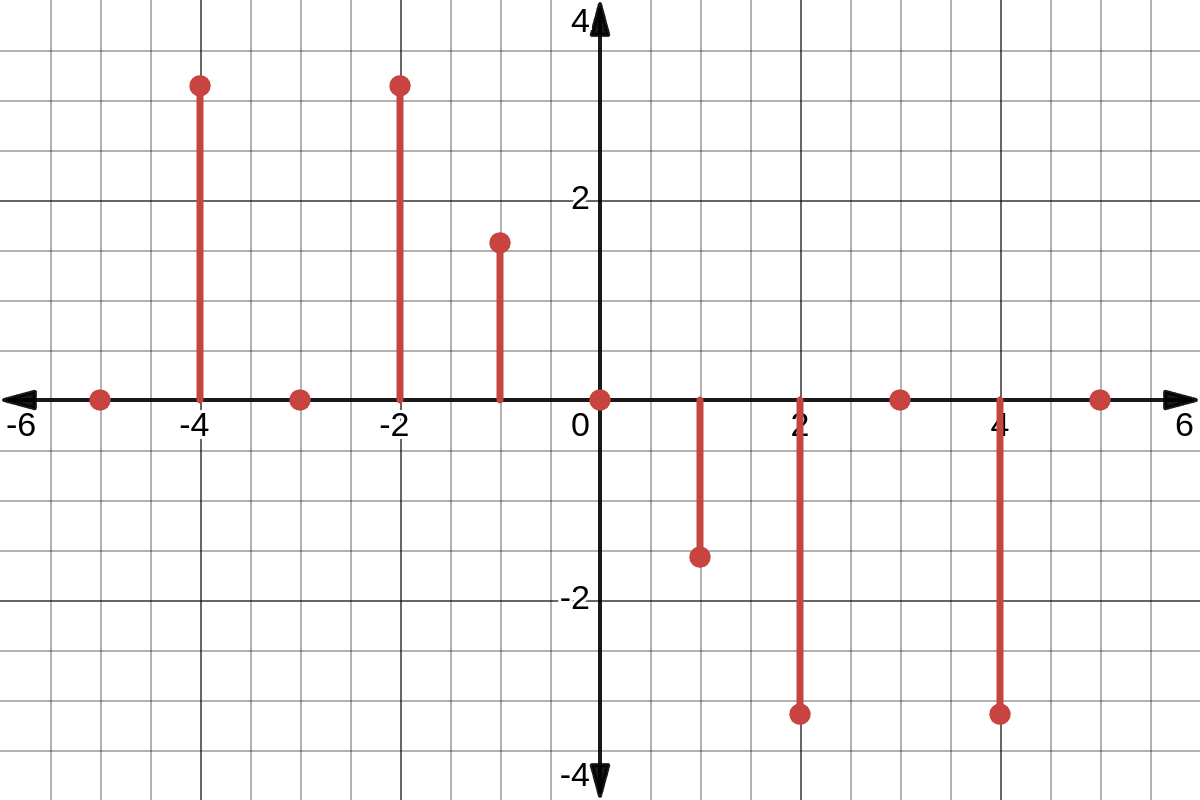
\includegraphics[width=1\textwidth]{images/ej2.4.png}	
      %graficos arg cn señal 2

      \item Considerar $|n| \leq 5$ y realizar el espectro de frecuencias de ambas señales en módulo, esto es, graficar 
        los pares ordenados

      $$\{(n, |C_n|) \mid -5 \leq n \leq 5\}$$

      correspondientes a cada señal $x_1, x_2$.\newline

  \textbf{Señal $x_1$}\\
    
      Como los coeficientes \( b_{n} \) son todos 0, las fases de los coeficientes son:

  $$
    \begin{aligned}
      \angle C_{n} &= \pi \quad \text{para} \quad n > 0 \\
      \angle C_{n} &= 0 \quad \text{para} \quad n = 0 \\
      \angle C_{n} &= \pi \quad \text{para} \quad n < 0
    \end{aligned}
  $$

%incluir imagen ej.2.5

      \textbf{Señal $x_2$}\\
      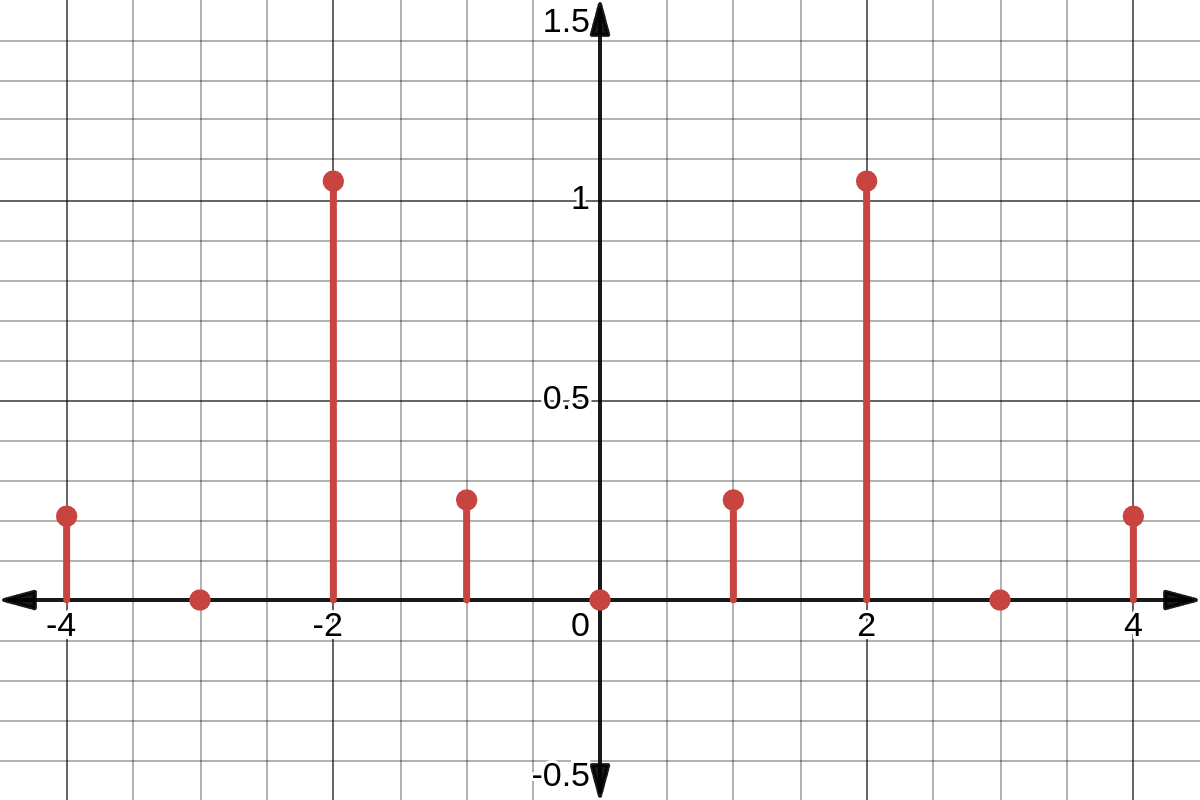
\includegraphics[width=1\textwidth]{images/ej2.6.png}	\\

      %graficos amplitud señal 2


    \item Calcular una aproximación a las potencias medias $P_1, P_2$, por medio de la relación de Parseval con los 
      espectros de frecuencia de ambas señales en módulo (usar la información de los incisos anteriores) y discriminar 
      el aporte de las componentes (CC, AC).

	Potencia media por medio de Parseval:
	$$
	P_m=\sum^\infty_{-\infty}|C_n|^2
	$$
            Si truncamos la suma, obtenemos una aproximación de la misma, en este caso la truncamos en n=5\\

  \textbf{Señal $x_1$}
  $$
  | \frac{2}{\pi } |^{2} +2|\frac{4}{3\pi } |^{2} +2|\frac{4}{15\pi } |^{2} +2|\frac{4}{35\pi } |^{2} +2|\frac{4}{63\pi } |^{2} +2|\frac{4}{99\pi } |^{2} \approx \frac{1}{2}
  $$
          
	\textbf{Señal $x_2$}
	$$
	P_m=\sum^5_{-5}|C_n|^2=|\frac{1}{\pi}|^2+2|\frac{j}{4}|^2+2|-\frac{1}{3\pi}|^2+2|-\frac{1}{15\pi}|^2
	$$
            
	$$
	=\frac{1}{\pi^2}+\frac{1}{16}+\frac{1}{9\pi^2}+\frac{1}{225\pi^2}\approx 0.2497 \approx 0.25
	$$
	El aporte del componente es de $\frac{1}{\pi^2}\approx0.101$ y el del componente AC es $P_m-DC\approx 0.1484$


      \textbf{Reflexionar:} ¿Qué ventajas/desventajas encuentra entre el método directo para calcular la potencia media 
      $P_1, P_2$ de las señales $x_1, x_2$ en la variable de tiempo $t$ y el método que se deriva de la relación de 
      Parseval, en donde los cálculos se realizan en la variable $n \in \mathbb{Z}$?

      Con el método directo puede ocurrir que calcular la potencia no sea sencillo debido a la forma analítica de
      la función en el dominio del tiempo, y además no hay información del aporte de cada armónico en la potencia 
      de la señal.  
  \end{itemize}

  \item Comparar los espectros obtenidos para cada una de las señales $x_1, x_2$, evaluar y proponer las 
    características sobresalientes de ambos espectros.\\
    El espectro de amplitud-frecuencia muestra que el aporte de los 
    primeros armónicos tienen mayor relevancia en ambas señales, sin
    embargo los armónicos pares en la señal rectificada de media onda 
    desaparece. En el espectro de fase-frecuencia observamos que en 
    la señal rectificada de onda completa todos los armonicos tienen 
    un desfase en $\pi$, en cambio en la señal rectificada de media onda 
    los armónicos tienen un desfase de $\pi$ para los n pares, y 0 para 
    los impares, excepto en $n=-1,1$, en los cuales el desfase es $\frac{\pi}{2}$ y $\frac{-\pi}{2}$, respectivamente.

\end{enumerate}

\chapter{}%ejercicio 3

Considerar $G_T(t) = \mu_{(t + \frac{T}{2})} - \mu_{(t - \frac{T}{2})}$ una señal pulso rectangular con duración finita
$T$ y amplitud unitaria.

\begin{enumerate}[label=\alph*),left=0pt]

  \item Realizar el gráfico de las señales $x_1 = G_1(t)$ y $x_2 = G_{0.1}(t)$, luego, calcular la energía $E_1$ de 
    $x_1$, y similarmente $E_2$ de $x_2$.

    \begin{figure}[h!]
      \hspace{6mm}
      \begin{minipage}{0.45\textwidth}
        \centering
        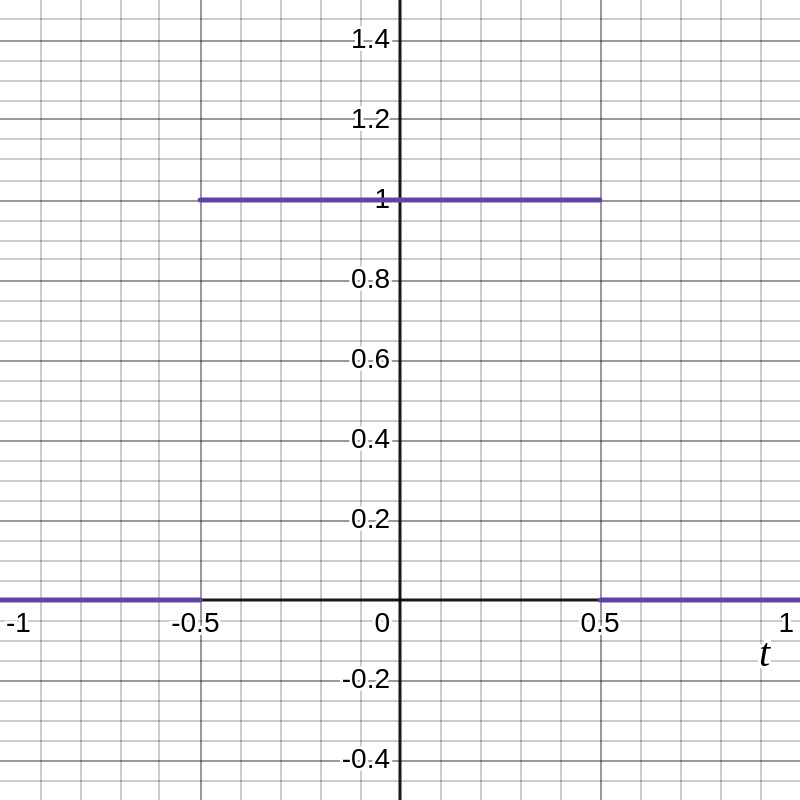
\includegraphics[width=\textwidth]{images/ej3.1}
        \caption{Grafico de la señal $x_1$}
        \label{fig:imagen1}
      \end{minipage}
      \hfill
      \begin{minipage}{0.45\textwidth}
        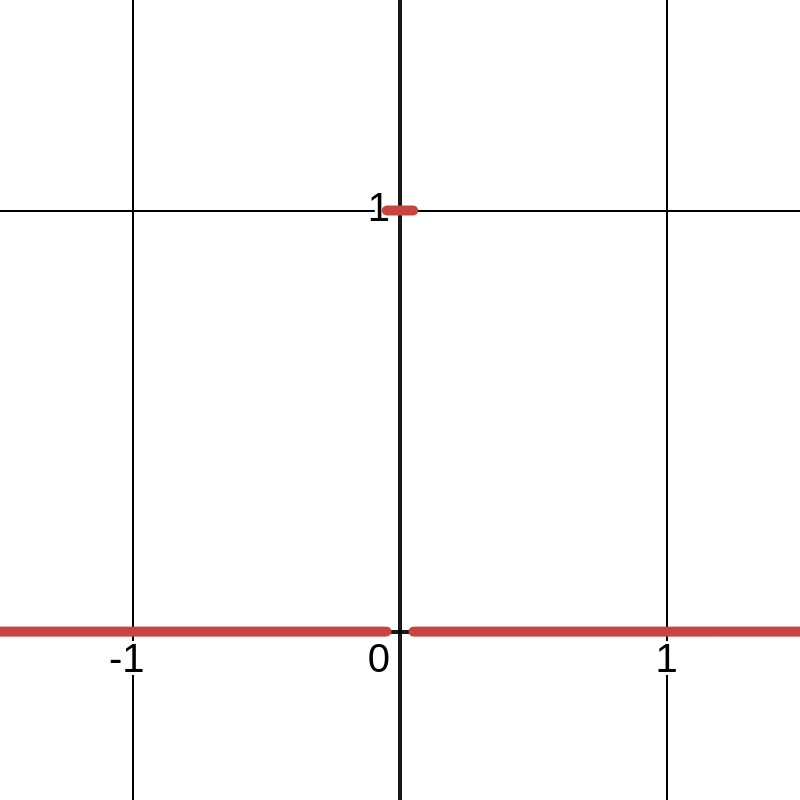
\includegraphics[width=\textwidth]{images/ej3.2}
        \caption{Grafico de la señal $x_2$}
        \label{fig:imagen2}
      \end{minipage}
    \end{figure}

    Para calcular la energia de cada respectiva señal aplicamos la definición:
    $$E_x = \int_{-\infty}^{\infty}x_t^2dt$$
    En este caso, por ser una señal de amplitud 1, simplemente es el area encerrada bajo cada una de las curvas
    $$E_1 = \int_{-\infty}^{\infty}x_1^2dt= \int_{-0,5}^{0,5}1dt=1$$
    $$E_2 = \int_{-\infty}^{\infty}x_2^2dt= \int_{-0,05}^{0,05}1dt=0.1$$

  \item Obtener la transformada de Fourier $F_1(\omega) = \mathcal{F}\{x_1\}$ y similarmente $F_2(\omega) =
    \mathcal{F}\{x_2\}$. \textbf{Reflexionar:} ¿En qué variable están definidas las funciones $F_1, F_2$?
    ¿Qué representa la variable $\omega$ y qué diferencia tiene con la variable $t$? 
    ¿Las funciones $F_1, F_2$ resultan periódicas?

    La transformada de furier para una un pulso genérico $G_T$ es:

    $$\mathcal{F}\{G_T\} = \int_{-\infty}^{\infty}G_T e^{-jwt}dt$$

    Pero, como $G_T$ es 1 en el intervalo $(-\frac{T}{2},\frac{T}{2})$ y 0 en el resto.

    $$
    \begin{aligned}
      \mathcal{F}\{G_T\} &= \int_{-\frac{T}{2}}^{\frac{T}{2}}e^{-jwt}dt \\[6pt]
      \mathcal{F}\{G_T\} &= -\frac{e^{-jwt}}{jw}\Big|^{\frac{T}{2}}_{-\frac{T}{2}} \\[6pt]
      \mathcal{F}\{G_T\} &= -\frac{e^{\frac{-jwT}{2}}-e^{\frac{jwT}{2}}}{jw}\\[6pt]
      \text{como:} \hspace{2mm} sin(&x)=\frac{e^{jx}-e^{-jx}}{2j}\\[6pt]
      \mathcal{F}\{G_T\} &= \frac{2}{w}sin\Big(\frac{wT}{2}\Big)
    \end{aligned}
    $$

    Por ende para la señal $x_1$ la transformada será:
    $$F_1= \frac{2}{w}sin\Big(\frac{w}{2}\Big)$$

    Y para $x_2$ la transformada será:
    $$F_1= \frac{2}{w}sin\Big(\frac{w}{20}\Big)$$

    \begin {itemize}[left=0pt]

      \item Graficar el espectro de frecuencia en fase para $F_1, F_2$, esto es, graficar los pares ordenados
        $$\{(\omega, \text{Arg}(F)) \mid \omega \in \mathbb{R}\}$$
        Para cada una de las funciones $F_1, F_2$.\newline

        \begin{figure}[h!]
          \hspace{10mm}
          \begin{minipage}{0.45\textwidth}
            \centering
            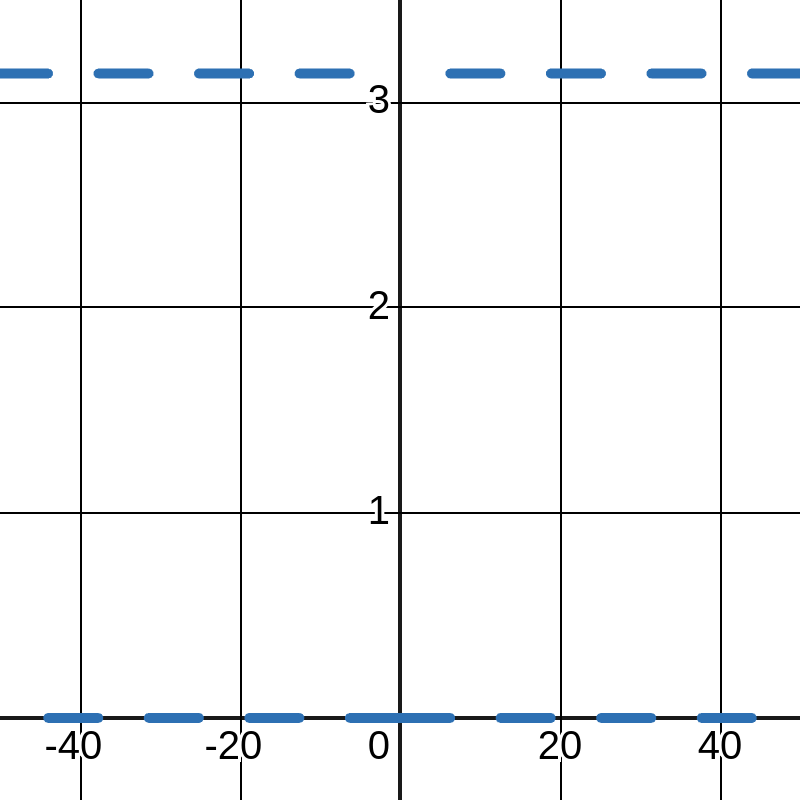
\includegraphics[width=\textwidth]{images/ej3.3}
            \caption{Espectro de frecuencia en fase para $x_1$}
            \label{fig:imagen1}
          \end{minipage}
          \hfill
          \begin{minipage}{0.45\textwidth}
            \centering
            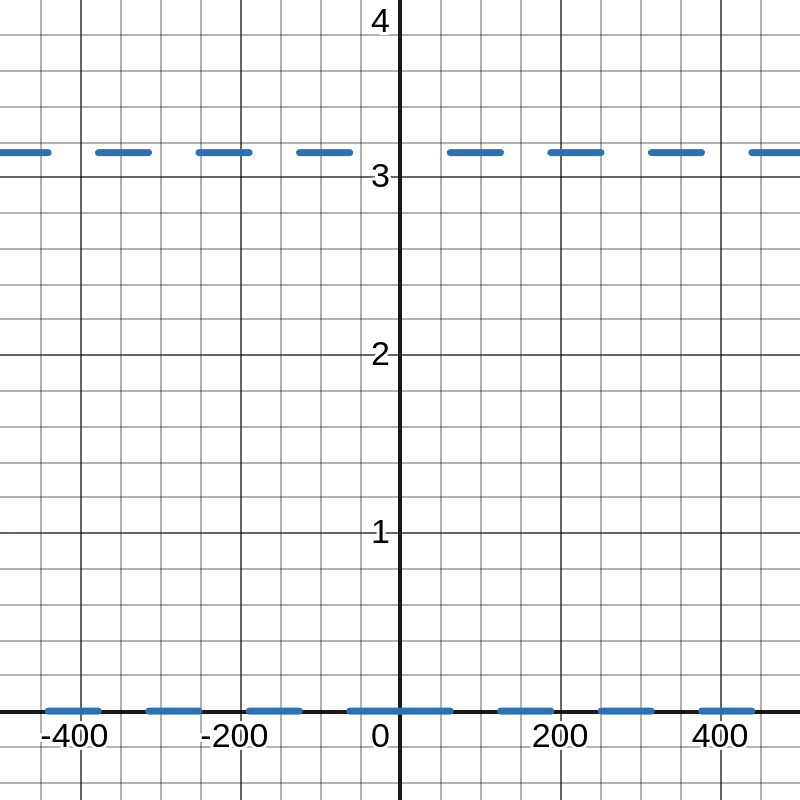
\includegraphics[width=\textwidth]{images/ej3.4}
            \caption{Espectro de frecuencia en fase para $x_2$}
            \label{fig:imagen2}
          \end{minipage}
        \end{figure}

        \textbf{Reflexionar:} ¿El espectro de frecuencia en fase es discreto o continuo? ¿El gráfico admite una simetría
        par, impar o ninguna?\\

        En ambos casos, el espectro de la frecuencia en fase es una señal de tiempo continuo y admite simetria par.\\

      \item Graficar el espectro de frecuencia en módulo para $F_1, F_2$, esto es, graficar los pares ordenados
        $$\{(\omega, |F|) \mid \omega \in \mathbb{R}\}$$
        Para cada una de las funciones $F_1, F_2$.\newline

        \begin{figure}[h!]
          \hspace{10mm}
          \begin{minipage}{0.45\textwidth}
            \centering
            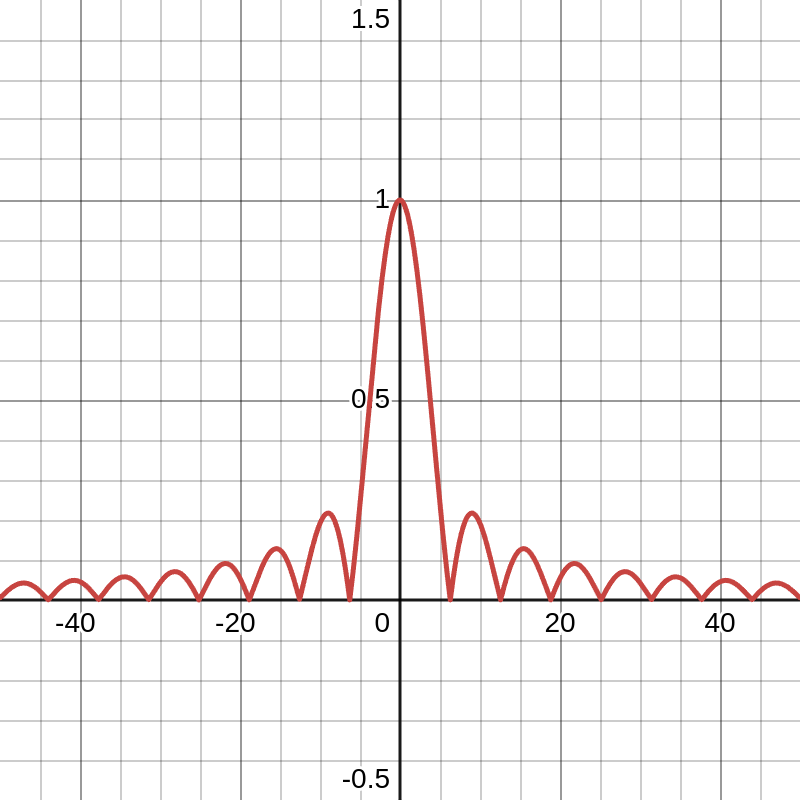
\includegraphics[width=\textwidth]{images/ej3.5}
            \caption{Espectro de frecuencia en módulo para $x_1$}
            \label{fig:imagen1}
          \end{minipage}
          \hfill
          \begin{minipage}{0.45\textwidth}
            \centering
            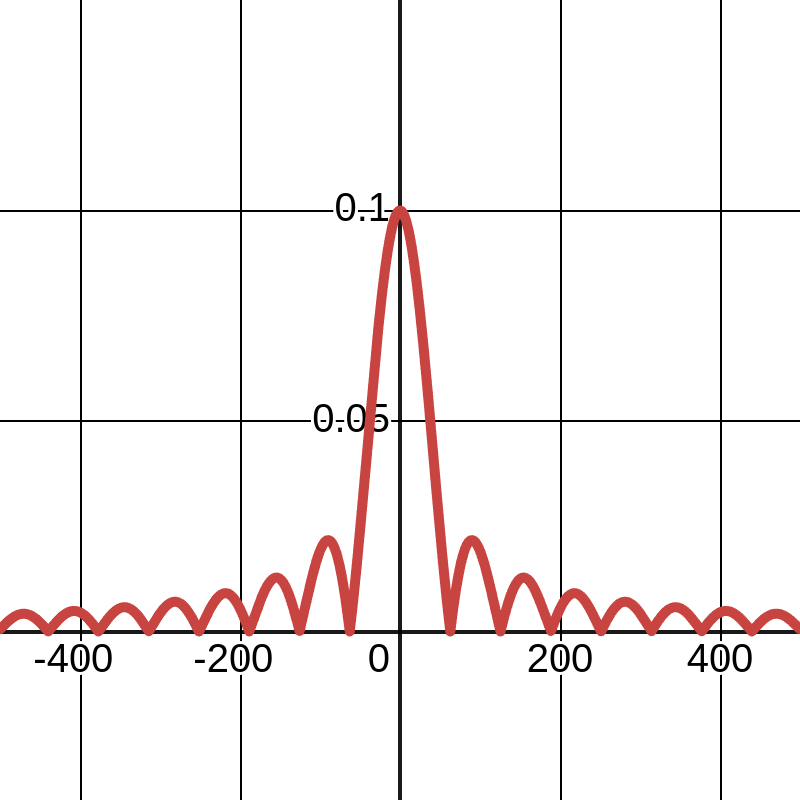
\includegraphics[width=\textwidth]{images/ej3.6}
            \caption{Espectro de frecuencia en módulo para $x_2$}
            \label{fig:imagen2}
          \end{minipage}
        \end{figure}

        \textbf{Reflexionar:} ¿El espectro de frecuencia en módulo es discreto o continuo? ¿El gráfico admite una 
        simetría par, impar o ninguna?\\

        Para ambas señales el espectro de frecuencia en modulo es una señal de tiempo continuo, y admiten simtria par.\\

      \item Graficar la densidad espectral para $F_1, F_2$, esto es, graficar los pares ordenados
        $$\{(\omega, |F|^2) \mid \omega \in \mathbb{R}\}$$
        Para cada una de las funciones $F_1$, $F_2$.\\

        \begin{figure}[h!]
          \hspace{10mm}
          \begin{minipage}{0.45\textwidth}
            \centering
            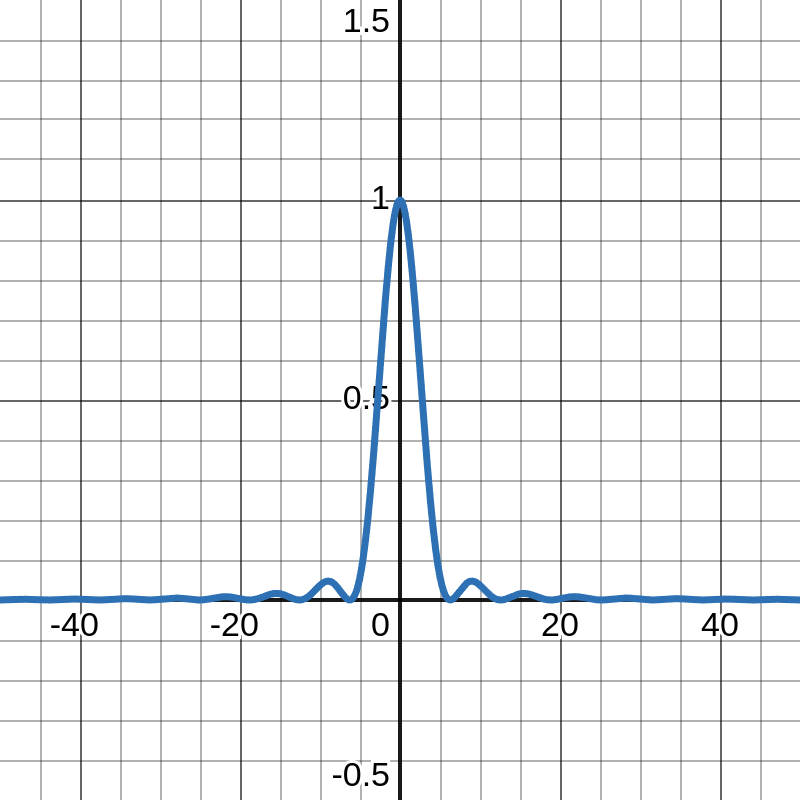
\includegraphics[width=\textwidth]{images/ej3.7}
            \caption{Densidad espectral para $x_1$}
            \label{fig:imagen1}
          \end{minipage}
          \hfill
          \begin{minipage}{0.45\textwidth}
            \centering
            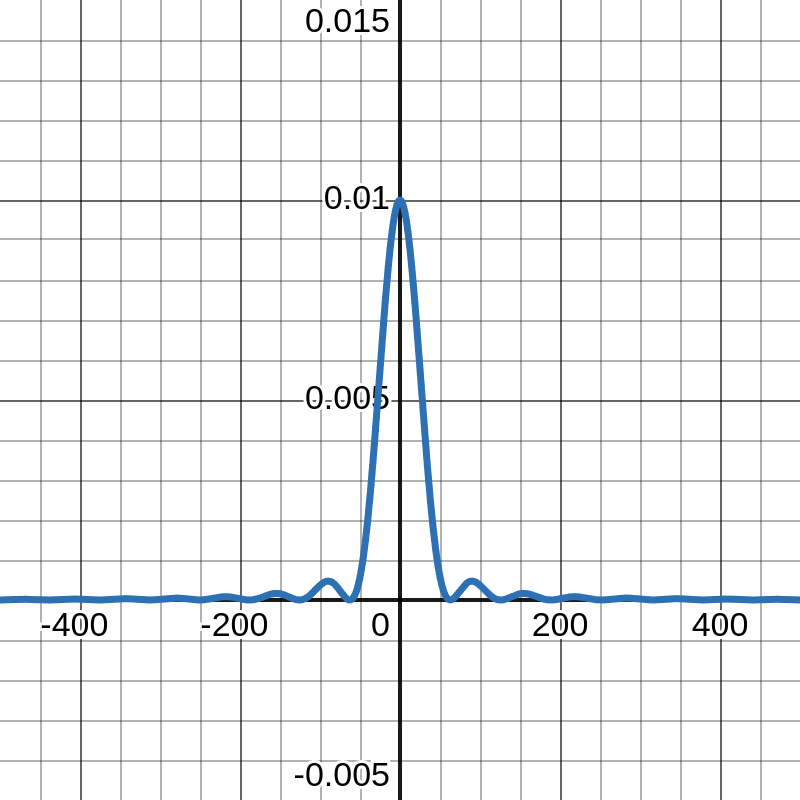
\includegraphics[width=\textwidth]{images/ej3.8}
            \caption{Densidad espectral para $x_2$}
            \label{fig:imagen2}
          \end{minipage}
        \end{figure}

        \textbf{Reflexionar:} ¿La densidad espectral es discreta o continua? ¿El gráfico admite una simetría par, impar
        o ninguna?\\

        La densidad espectral tambien es una señal de tiempo continuo, y acepta simetria par.\\

      \item Calcular la energía $E_1, E_2$ haciendo uso de la relación de Parseval.

        La relacion de Parseval indica que:

        $$E_x=\frac{1}{2\pi}\int_{-\infty}^{\infty}|\mathcal{F}\{x\}|^2$$

        Primero resolveremos la integral:
        $$
        \begin{aligned}
          \int_{-\infty}^{\infty} \Bigg[\hspace{1mm}\frac{2}{\omega} \sin\left(\frac{\omega T}{2}\right)\Bigg]^2 d\omega
          &=\int_{-\infty}^{\infty} \frac{4}{\omega^2} \sin^2\left(\frac{\omega T}{2}\right) d\omega \\[6pt]
          &= \sin^2\left(\frac{\omega T}{2}\right) \Big(-\frac{4}{\omega}\Big) - \int_{-\infty}^{\infty} 
          \Big(-\frac{4}{\omega}\Big) \frac{T}{2} \sin(\omega T)d\omega \\[6pt]
          &= \sin^2\Big(\frac{\omega T}{2}\Big)\Big(-\frac{4}{\omega}\Big) +
            2 T^2 \int \frac{\sin(\omega T)}{\omega T}d\omega \\[6pt]
          &\text{Apoyandonos en la sustitución $\omega T=x$}\\[6pt]
          &=-\sin^2\Big(\frac{\omega T}{2}\Big)\frac{4}{\omega} + 2T \int_{-\infty}^{\infty} \frac{\sin(x)}{x} dx\\[6pt]
          &=\Big[-\frac{4}{\omega} \Big(\frac{1- \cos(\omega t)}{2}\Big) + 2T Si(x)\Big]\Big|_{-\infty}^{\infty}\\[6pt]
          &=\Big[\frac{2}{\omega} (\cos(wt) - 1) + 2T Si(\omega T)\Big]\Big|_{-\infty}^{\infty}\\[6pt]
        \end{aligned}
        $$

        Desarrollando el primer termino:
        $$
        \begin{aligned}
          2\frac{\cos(\omega T)-1}{\omega} \Big|_{-\infty}^{\infty}&=2\frac{\cos(\omega T)-1}{\omega} 
          \Big|_{-\infty}^{0} + 2\frac{\cos(\omega T)-1}{\omega} \Big|_{0}^{\infty}\\[6pt]
          &= 0
        \end{aligned}
        $$

        Desarrollando el segundo termino:
        $$
        \begin{aligned}
          2T\text{Si}(\omega T)\Big|_{-\infty}^{\infty} &=
          2T\text{Si}(\omega T)\Big|_{-\infty}^{0} + 2T\text{Si}(\omega T)
          \Big|_{0}^{\infty} \\[6pt]
          &= 2T(\text{Si}(0)-\lim_{\omega \to -\infty} \text{Si}(\omega T)) +
          2T(\lim_{\omega \to \infty} \text{Si}(\omega T) - \text{Si}(0))\\[6pt]
          &=  2T\frac{\pi}{2} + 2T \frac{\pi}{2} = 2\pi T
        \end{aligned}
        $$

        De esta forma podemos afirmar que:
        $$\int_{-\infty}^{\infty} \Bigg[\hspace{1mm}\frac{2}{\omega} 
        \sin\left(\frac{\omega T}{2}\right)\Bigg]^2 d\omega= 2\pi T$$

        Siendo la energía de cada señal a travez de la relacion de persaval:
          $$E_1 = \frac{2\pi \cdot 1}{2\pi} = 1 $$
          $$E_2 = \frac{2\pi \cdot 0.1}{2\pi} = 0.1 $$

        Esto coincidide con la energía calculada en el dominio del tiempo en el punto a.\\

        \textbf{Reflexionar:} ¿Qué ventajas/desventajas encuentra entre el método directo para calcular la energía $E_1,
        E_2$ de las señales $x_1, x_2$ en la variable de tiempo $t$ y el método que se deriva de la relación de Parseval
        , en donde los cálculos se realizan en la variable $\omega$?

        En este caso, el metodo sobre la variable $t$ es mucho mas simple, directo y visual. En contra parte el calculo
        mediante la relación de Parseval es mucho mas tedioso, requiriendo la resolucion de una integral compleja
        y la ayuda de herramientas como la función $Si()$. Sin embargo, esto se debe a las caracteristicas de nuestra
        señal en particular, es decir que no es extensible a otros casos.

  \end{itemize}

  \item Comparar los espectros obtenidos para cada una de las señales $x_1, x_2$, evaluar y proponer las 
    características sobresalientes de ambos espectros.

    Se puede observar claramente en los graficos que los espectros obtenidos obedecen a la relación:

    $$
    \begin{aligned}
      x(t) &\leftrightarrow X(w) \\[6pt]
      x(t\alpha) &\leftrightarrow \frac{1}{|\alpha|}X\Big(\frac{w}{\alpha}\Big)
    \end{aligned}
    $$

    Esto sugiere que, al ser $x_1$ más extensa en el tiempo y, por lo tanto, presentar cambios más suaves, su espectro
    estará concentrado en frecuencias más bajas en comparación con el espectro de la señal $x_2$. Esta última, al estar
    más acotada en el tiempo y variar más rápidamente, mostrará un espectro con componentes de frecuencias más altas.

\end{enumerate}

\chapter{}%ejercicio 4

  \textbf{Circuito Eléctrico RC:} circuito eléctrico correspondiente a un sistema de 1° orden y su ecuación
  característica:
  $$v(t) = R\cdot i(t) + \frac{1}{C} \cdot \int_{0}^{t} i(\tau) d\tau$$

  \vspace{-1cm}
  \noindent
  \begin{figure}[h]
    \centering
    \begin{minipage}[h]{0.5\textwidth}
      \centering
      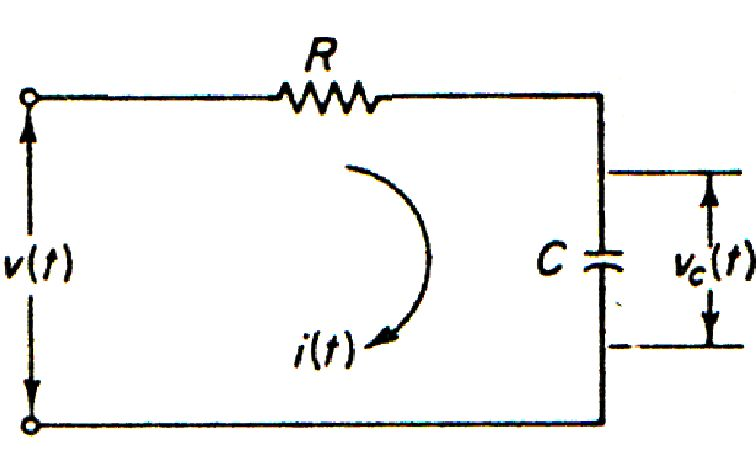
\includegraphics[width=1\textwidth]{./images/ej4.1.jpg}
      \textit{Circuito RC}
    \end{minipage}
  \end{figure}

  \begin{enumerate}[label=\alph*)]
    \item Obtener una representación del circuito con Ecuaciones Diferenciales de primer orden y coeficientes
      constantes, y con ello, definir un Sistema en tiempo continuo con entrada $x(t) = v(t)$ y salida $y(t) = i(t)$.
      Luego, hacer un diagrama de bloques de la E.D; exponiendo los integradores que la conforma.

      El circuito RC esta descrito por la ecuacion caracteristica:
      $$v(t) = R\cdot i(t) + \frac{1}{C} \cdot \int_{0}^{t} i(\tau) d\tau$$
      Para tener una nomenclatura mas generica, sustituimos la entrada $v(t)$ con $x(t)$ y la salida $i(t)$ con $y(t)$:
      $$x(t) = R\cdot y(t) + \frac{1}{C} \cdot \int_{0}^{t} y(\tau) d\tau$$
      Teniendo en cuenta que $y(t)$ es la salida e $x(t)$ la entrada, las ecuaciones diferenciales toman la forma:
      $$\left(D^N + \sum_{i=0}^{N-1} a_i D^i\right) \cdot y(t) = \left(\sum_{i=0}^{M} b_i D^i\right) \cdot x(t)$$
      Reacomodando la ecuacion caracteristica generalizada, nos queda:
      $$
      \begin{aligned}
        y(t) + D^{-1} \left\{\frac{1}{RC} \cdot y(t) \right\} &= x(t) \cdot \frac{1}{R}\\[6pt]
        D^1\Bigl\{y(t) \Bigl\} + \frac{1}{RC} \cdot y(t) &= D^1\left\{x(t) \cdot \frac{1}{R} \right\}\\[6pt]
        \frac{dy(t)}{dt} + \frac{1}{RC} \cdot y(t) &= \frac{dx(t)}{dt} \cdot \frac{1}{R}\\[6pt]
      \end{aligned}
      $$

      Lo cual es la ecuacion diferencial de primer orden a coeficientes constantes que describe el comportamiento del
      circuito RC.

      Para el diagrama de simulacion, utilizamos la ecuacion caracteristica generalizada del sistema, solo que se
      despeja y:
      \begin{figure}[h]
        \centering
        \begin{tikzpicture}[auto, node distance=2cm, >=Stealth, thick]
          % Definición de estilos para los bloques y sumador
          \tikzstyle{block} = [draw, rectangle, minimum height=1.5em, minimum width=3em]
          \tikzstyle{sum} = [draw, circle, inner sep=1pt, minimum size=1cm, node distance=2cm]
          \tikzstyle{connector} = [fill, circle, minimum size=4pt, inner sep=0pt] % Estilo para el punto de conexión

          % Definición de nodos
          \node at (0,0) [coordinate] (input) {}; % Nodo de entrada
          \node [coordinate, right=7cm of input] (elbow1) {};
          \node [block, below=1cm of elbow1] (gain1) {$\frac{1}{R}$};
          \node [sum, below=1cm of gain1] (sum) {$+$};
          \node [block, left=2cm of sum] (integrator) {$\int$};
          \node [coordinate, left=2cm of integrator] (elbow2) {};
          \node [block, below=1cm of elbow2] (gain2) {$-\frac{1}{RC}$};
          \node [coordinate, below=1cm of gain2] (elbow3) {};
          \node [coordinate, right=4cm of sum] (output) {}; % Nodo de salida
          \node [connector, left=2cm of output] (elbow5) {};
          \node [coordinate, below=2.7cm of elbow5] (elbow4) {};

          % Conexiones entre nodos
          \draw [-] (input) -- node {$x(t)$} (elbow1);
          \draw [-] (elbow1) -- (gain1);
          \draw [->] (gain1) -- (sum);
          \draw [->] (sum) -- node {$y(t)$} (output);
          \draw [->] (integrator) -- (sum);
          \draw [->] (elbow2) -- (integrator);
          \draw [-] (gain2) -- (elbow2);
          \draw [->] (elbow3) -- (gain2);
          \draw [-] (elbow4) -- (elbow3);
          \draw [-] (elbow5) -- (elbow4);
        \end{tikzpicture}
        $$y_t = \frac{x_t}{R} + D^{-1}\left\{-\frac{y_t}{RC}\right\}$$
      \end{figure}

    \item Teniendo en cuenta el siguiente resultado matemático, obtener una descripción explicita
      de la respuesta $y(t)$ del sistema obtenido en el inciso anterior:
      \begin{itemize}
        \item Sean $\alpha, \beta_0, \beta_1 \in \mathbb{R}$ constantes; $y(t), x(t)$ funciones con variable de tiempo
        continuo,
          las cuales verifican la ecuación diferencial de primer orden con coeficientes constantes:

          $$y_t'+\alpha y_t = \beta_1 x_t' + \beta_0 x_t$$

          Entonces, una Solución General explicita de la Ecuación Diferencial es

          $$y_t = \beta_1 x_t + (y_0 - \beta_1 x_0) e^{-\alpha t} + (\beta_0 - \alpha \beta_1) \int_{0}^{t} x(\tau)
          e^{-\alpha(t - \tau)} d\tau$$

          donde $y_0 = y(0), x_0 = x(0)$ son Condiciones Iniciales arbitrarias
        \end{itemize}

        Identificando los coeficientes $\alpha, \beta_0, \beta_1$, tenemos lo siguiente:
        $$\alpha = \frac{1}{RC}; \hspace{1cm}\beta_0 = 0; \hspace{1cm}\beta_1 = \frac{1}{R}$$
        Por lo tanto, la solucion general explicita para el $S_1\{x_t\}$ es:
        $$y_t = S_1\{x_t\} = x_t \cdot \frac{1}{R} + \left(y_o - \frac{x_0}{R}\right) \cdot e^{\frac{-t}{RC}} -
        \frac{1}{R^2C} \int_{0}^{t} x_\tau \cdot e^{\frac{-(t-\tau)}{RC}} d\tau$$


    \item Usando la descripción explicita de la salida del Sistema $y_t = S_1{x_t}$ (CI arbitrarias) del inciso
      anterior, calcular la respuesta a cada una de las siguientes señales:
      $$x_0(t) = 0, \hspace{0.5cm}x_1(t) = \mu_t, \hspace{0.5cm}x_2(t) = \mu(t - t_0), \hspace{0.5cm}x_3(t) =
      \mu_t - \mu(t - t_0), \hspace{0.5cm}x_4(t) = t$$

      \textbf{Reflexionar:} ¿La señal $y_0$ es completamente nula? ¿Las señales $y_3, y' = y_1 - y_2$ (iguales o
      distintas)? ¿es suficiente para garantizar la Linealidad del sistema? ¿Las señales $y_1, y_2$ son iguales? ¿es
      suficiente para garantizar la Inv. Tiempo del sistema?.

      Solucion para $x_t = x_0 = 0$:
      \begin{align*}
        y_0(t) &= 0 \cdot \frac{1}{R} + \left(y_0 - \frac{x_0}{R}\right) \cdot
          e^{\frac{-t}{RC}} - \frac{1}{R^2C} \int_{0}^{t} 0 \cdot e^{\frac{-(t-\tau)}{RC}} d\tau\\[6pt]
        y_0(t) &= \left(y_0 - \frac{x_0}{R}\right) \cdot e^{\frac{-t}{RC}}
      \end{align*}
      Como se puede ver, la señal $y_0$ no es completamente nula. Esta presenta una exponencial decreciente para
      $t > 0$. Seria nula en caso de que las C.I. sean nulas, o que se cumpla que $y_0 = x_0/R$.\\

      Solucion para $x_t = x_1 = \mu_t$:
      \begin{align*}
        y_1(t) &= \mu_t \cdot \frac{1}{R} + \left(y_0 - \frac{x_0}{R}\right) \cdot
          e^{\frac{-t}{RC}} - \frac{1}{R^2C} \int_{0}^{t} \mu_t \cdot e^{\frac{-(t-\tau)}{RC}} d\tau\\[6pt]
        y_1(t) &= \mu_t \cdot \frac{1}{R} + \left(y_0 - \frac{x_0}{R}\right) \cdot e^{\frac{-t}{RC}} -
          \frac{1}{R^2C} \int_{0}^{t} e^v \cdot RCdv\\[6pt]
        y_1(t) &= \mu_t \cdot \frac{1}{R} + \left(y_0 - \frac{x_0}{R}\right) \cdot e^{\frac{-t}{RC}} -
          \frac{1}{R} \left[e^{\frac{-(t-\tau)}{RC}}\right]\Big|_{0}^{t}\\[6pt]
        y_1(t) &= \mu_t \cdot \frac{1}{R} + \left(y_0 - \frac{x_0}{R}\right) \cdot e^{\frac{-t}{RC}} - \frac{1}{R}
          \left[1 - e^{\frac{-t}{RC}}\right]
      \end{align*}
      Solucion para $x_t = x_2 = \mu_{t-1}$:
      \begin{align*}
        y_2(t) &= \mu_{t-1} \cdot \frac{1}{R} + \left(y_0 - \frac{x_0}{R}\right) \cdot
          e^{\frac{-t}{RC}} - \frac{1}{R^2C} \int_{0}^{t} \mu_{t-1} \cdot e^{\frac{-(t-\tau)}{RC}} d\tau\\[6pt]
        y_2(t) &= \mu_{t-1} \cdot \frac{1}{R} + \left(y_0 - \frac{x_0}{R}\right) \cdot e^{\frac{-t}{RC}} -
          \frac{1}{R^2C} \int_{1}^{t} e^v \cdot RCdv\\[6pt]
        y_2(t) &= \mu_{t-1} \cdot \frac{1}{R} + \left(y_0 - \frac{x_0}{R}\right) \cdot e^{\frac{-t}{RC}} -
          \frac{1}{R} \left[e^{\frac{-(t-\tau)}{RC}}\right]\Big|_{1}^{t}\\[6pt]
        y_2(t) &= \mu_{t-1} \cdot \frac{1}{R} + \left(y_0 - \frac{x_0}{R}\right) \cdot e^{\frac{-t}{RC}} -
          \frac{1}{R} \left[1 - e^{\frac{1-t}{RC}}\right]
      \end{align*}
      Solucion para $x_t = x_3 = \mu_t - \mu_{t-1}$:
      \begin{align*}
        y_3(t) &= (\mu_t - \mu_{t-1}) \cdot \frac{1}{R} + \left(y_0 - \frac{x_0}{R}\right) \cdot e^{\frac{-t}{RC}} -
          \frac{1}{R^2C} \int_{0}^{t} (\mu_t - \mu_{t-1}) \cdot e^{\frac{-(t-\tau)}{RC}} d\tau\\[6pt]
        y_3(t) &= (\mu_t - \mu_{t-1}) \cdot \frac{1}{R} + \left(y_0 - \frac{x_0}{R}\right) \cdot e^{\frac{-t}{RC}} -
          \frac{1}{R^2C} \left[\int_{0}^{t} \mu_t \cdot e^{\frac{-(t-\tau)}{RC}} d\tau -
          \int_{0}^{t} \mu_{t-1} \cdot e^{\frac{-(t-\tau)}{RC}} d\tau \right]\\[6pt]
        y_3(t) &= (\mu_t - \mu_{t-1}) \cdot \frac{1}{R} + \left(y_0 - \frac{x_0}{R}\right) \cdot e^{\frac{-t}{RC}} -
        \frac{1}{R^2C} \left[\int_{0}^{t} e^{\frac{-(t-\tau)}{RC}} d\tau -
          \int_{1}^{t} e^{\frac{-(t-\tau)}{RC}} d\tau \right]\\[6pt]
        y_3(t) &= (\mu_t - \mu_{t-1}) \cdot \frac{1}{R} + \left(y_0 - \frac{x_0}{R}\right) \cdot e^{\frac{-t}{RC}} -
          \frac{1}{R^2C} RC\left[\int_{0}^{t} e^v dv - \int_{1}^{t} e^v dv \right]\\[6pt]
        y_3(t) &= (\mu_t - \mu_{t-1}) \cdot \frac{1}{R} + \left(y_0 - \frac{x_0}{R}\right) \cdot e^{\frac{-t}{RC}} -
          \frac{1}{R}\left[e^{\frac{-(t-\tau)}{RC}} \Big|_{0}^{t} -
          e^{\frac{-(t-\tau)}{RC}} \Big|_{1}^{t} \right]\\[6pt]
        y_3(t) &= (\mu_t - \mu_{t-1}) \cdot \frac{1}{R} + \left(y_0 - \frac{x_0}{R}\right) \cdot e^{\frac{-t}{RC}} -
          \frac{1}{R} \left[e^{\frac{1-t}{RC}} - e^{\frac{-t}{RC}}\right]
      \end{align*}
      Solucion para $y' = y_1 - y_2$:
      \begin{align*}
        y' &= \mu_t \cdot \frac{1}{R} + \left(y_0 - \frac{x_0}{R}\right) \cdot e^{\frac{-t}{RC}} - \frac{1}{R}
          \left[1 - e^{\frac{-t}{RC}}\right] - \left(\mu_{t-1} \cdot \frac{1}{R} + \left(y_0 -
          \frac{x_0}{R}\right) \cdot e^{\frac{-t}{RC}} - \frac{1}{R} \left[1 - e^{\frac{1-t}{RC}}\right]\right)\\[6pt]
        y' &= (\mu_t - \mu_{t-1}) \cdot \frac{1}{R} - \frac{1}{R} \left[e^{\frac{1-t}{RC}} - e^{\frac{-t}{RC}}\right]
      \end{align*}
      Como se puede ver, $y' \neq y_3$. Esto significa que el sistema $S_1\left\{x_t\right\}$ no es lineal. Se puede
      ver que si las condiciones lineales son nulas, o si $y_0 = x_0/R$, la igualdad se cumple, y el sistema es lineal.
      Por otro lado, las ecuaciones $y_1 \neq y_2$, ademas, con ellas no se puede demostrar la invarianza en el tiempo,
      debido a que por un lado, se debe desplazar la señal de entrada, y por otro lado, se debe desplazar la señal de
      salida, para verificar que el sistema es invariante en el tiempo.\\

      Solucion para $x_t = x_4 = t$:
      \begin{align*}
        y_4(t) &= t \cdot \frac{1}{R} + \left(y_0 - \frac{x_0}{R}\right) \cdot e^{\frac{-t}{RC}} -
          \frac{1}{R^2C} \int_{0}^{t} \tau \cdot e^{\frac{-(t-\tau)}{RC}} d\tau\\[6pt]
        y_4(t) &= t \cdot \frac{1}{R} + \left(y_0 - \frac{x_0}{R}\right) \cdot e^{\frac{-t}{RC}} -
          \frac{1}{R^2C} \left[\tau \cdot RC e^{\frac{-(t-\tau)}{RC}} - RC\int e^{\frac{-(t-\tau)}{RC}} d\tau\right]
          \Big|_{0}^{t}\\[6pt]
        y_4(t) &= t \cdot \frac{1}{R} + \left(y_0 - \frac{x_0}{R}\right) \cdot e^{\frac{-t}{RC}} -
          \frac{1}{R} \left[\tau \cdot e^{\frac{-(t-\tau)}{RC}} - RC\int e^v dv\right] \Big|_{0}^{t}\\[6pt]
        y_4(t) &= t \cdot \frac{1}{R} + \left(y_0 - \frac{x_0}{R}\right) \cdot e^{\frac{-t}{RC}} -
          \frac{1}{R} \left[\tau \cdot e^{\frac{-(t-\tau)}{RC}} - RC e^{\frac{-(t-\tau)}{RC}} \right]
          \Big|_{0}^{t}\\[6pt]
        y_4(t) &= t \cdot \frac{1}{R} + \left(y_0 - \frac{x_0}{R}\right) \cdot e^{\frac{-t}{RC}} -
          \frac{1}{R} \left[e^{\frac{-(t-\tau)}{RC}} (\tau - RC)\right] \Big|_{0}^{t}\\[6pt]
        y_4(t) &= t \cdot \frac{1}{R} + \left(y_0 - \frac{x_0}{R}\right) \cdot e^{\frac{-t}{RC}} -
          \frac{1}{R} \left[t - RC + RC e^{\frac{-t}{RC}}\right]\\[6pt]
      \end{align*}

    \item Usando la descripción explicita de la salida del Sistema $y_t = S_1\{x_t\}$ (CI arbitrarias), demostrar si el
      Sistema $S_1$ es (o no): Lineal, Homogéneo e Invariante en el Tiempo.

      \textbf{Linealidad:} La verificacion de la linealidad del sistema, viene de la mano de la homogeneidad y la aditividad,
      los cuales se demuestran a continuacion, donde $x_a$ y $x_b$ son dos señales arbitrarias, e $y_1(t) = S_1\{k_0x_a\},
      y_2(t) = S_1\{k_0x_b\}$ y $y_3(t) = k_0S_1\{x_a + x_b\}$:
      \begin{align*}
        y_1(t) &= k_0x_a \cdot \frac{1}{R} + \left(y_0 - \frac{x_0}{R}\right) \cdot
          e^{\frac{-t}{RC}} - \frac{1}{R^2C} \int_{0}^{t} k_0x_a \cdot e^{\frac{-(t-\tau)}{RC}} d\tau\\[12pt]
        y_2(t) &= k_0x_b \cdot \frac{1}{R} + \left(y_0 - \frac{x_0}{R}\right) \cdot
          e^{\frac{-t}{RC}} - \frac{1}{R^2C} \int_{0}^{t} k_0x_b \cdot e^{\frac{-(t-\tau)}{RC}} d\tau\\[12pt]
        y_3(t) &= k_0\left((x_a + x_b) \cdot \frac{1}{R} + \left(y_0 - \frac{x_0}{R}\right) \cdot e^{\frac{-t}{RC}} -
          \frac{1}{R^2C} \int_{0}^{t} (x_a + x_b) \cdot e^{\frac{-(t-\tau)}{RC}} d\tau\right)\\[12pt]
        y_3(t) &= y_1(t) + y_2(t)\\[6pt]
        y_3(t) &\neq k_0(x_a + x_b) \cdot \frac{1}{R} + 2\left(y_0 - \frac{x_0}{R}\right) \cdot
          e^{\frac{-t}{RC}} - \frac{1}{R^2C} \int_{0}^{t} k_0(x_a + x_b) \cdot e^{\frac{-(t-\tau)}{RC}} d\tau
      \end{align*}
      La desigualdad anterior permite establecer que el $S_1\{x_t\}$ no es ni aditivo ni homogeneo, por lo tanto no es
      lineal. Esto se debe a causa del termino no lineal que involucra las condiciones iniciales.\\

      \textbf{Invarianza en el tiempo:} La verificacion de la invarianza en el tiempo involucra realizar un desplazamiento
      temporal en la señal de entrada, y comparar si realizando un desplazamiento temporal en la señal de salida, se
      obtiene la misma señal o no. Para eso, establecemos que $t_0$ es un desplazamiento arbitrario, que $y_1(t) = S_1
      \{x_{(t-t_0)}\}$ y que $y_2(t) = y_{(t-t_0)}$:
      \begin{align*}
        y_1(t) &= x_{(t - t_0)} \cdot \frac{1}{R} + \left(y_0 - \frac{x_0}{R}\right) \cdot
          e^{\frac{-t}{RC}} - \frac{1}{R^2C} \int_{0}^{t} x_{(\tau - t_0)} \cdot e^{\frac{-(t-\tau)}{RC}} d\tau\\[12pt]
        y_2(t) &= x_{(t - t_0)} \cdot \frac{1}{R} + \left(y_0 - \frac{x_0}{R}\right) \cdot e^{\frac{-(t-t_0)}{RC}} -
          \frac{1}{R^2C} \int_{0}^{t - t_0} x_{(\tau)} \cdot e^{\frac{-(t-t_0-\tau)}{RC}} d\tau\\[6pt]
        v &= t+\tau; \hspace{7mm} dv = d\tau; \hspace{7mm} \tau \rightarrow t-t_0, v \rightarrow t;
          \hspace{7mm} \tau \rightarrow 0, v \rightarrow t_0\\[6pt]
        y_2(t) &= x_{(t - t_0)} \cdot \frac{1}{R} + \left(y_0 - \frac{x_0}{R}\right) \cdot e^{\frac{-(t-t_0)}{RC}} -
          \frac{1}{R^2C} \int_{t_0}^{t} x_{(v-t_0)} \cdot e^{\frac{-(t-v)}{RC}} dv\\[12pt]
        &\hspace{4cm}y_1(t) \neq y_2(t)
      \end{align*}
      Como se puede ver, $y_1(t) \neq y_2(t)$, por lo que el $S_1\{x_t\}$ no es invariante en el tiempo. Esto es debido
      a los limites de integracion, ya que el resto de los terminos son practicamente iguales, y por el termino no
      lineal que involucra las condiciones iniciales.

    \item Demostrar que el sistema anterior en reposo gana propiedades, esto es, definir $y_t = S_2\{x_t\}$ con C.I. 
      nulas $y_0 = x_0 = 0$, y clasificar el sistema S2 (Aditivo, Homogéneo, Inv. Tiempo).

      La respuesta del sistema ahora esta dada por la ecuación:
      $$y(t) = x(t) \cdot \frac{1}{R}- \frac{1}{R^2C} \int_{0}^{t} x(\tau) \cdot e^{\frac{\tau-(t - t_0))}{RC}} d\tau$$

      \textbf{Linealidad:} Trayendo el analisis del punto anterior, tenemos que:
      \begin{align*}
        y_3(t) &= k_0\left((x_a + x_b) \cdot \frac{1}{R} + \left(y_0 - \frac{x_0}{R}\right) \cdot e^{\frac{-t}{RC}} -
          \frac{1}{R^2C} \int_{0}^{t} (x_a + x_b) \cdot e^{\frac{-(t-\tau)}{RC}} d\tau\right)\\[12pt]
        y_3(t) &= y_1(t) + y_2(t)\\[6pt]
        y_3(t) &\neq k_0(x_a + x_b) \cdot \frac{1}{R} + 2\left(y_0 - \frac{x_0}{R}\right) \cdot
          e^{\frac{-t}{RC}} - \frac{1}{R^2C} \int_{0}^{t} k_0(x_a + x_b) \cdot e^{\frac{-(t-\tau)}{RC}} d\tau
      \end{align*}
      Como ahora, para el $S_2$ las C.I. son nulas, la desigualdad ahora se cumple, quedando:
      \begin{gather*}
        y_3(t) = y_1(t) + y_2(t)\\[6pt]
        y_3(t) = k_0\left((x_a + x_b) \cdot \frac{1}{R} - \frac{1}{R^2C} \int_{0}^{t} (x_a + x_b) \cdot
        e^{\frac{-(t-\tau)}{RC}} d\tau\right)
      \end{gather*}
      Lo cual verifica que el $S_2$ es completamente aditivo y homogeneo, por lo que ahora se lo puede considerar
      lineal.\\

      \textbf{Invarianza en el tiempo:} La respuesta del sistema desplazada $t_0$ es:
      $$y(t - t_0) = x(t - t_0) \cdot \frac{1}{R}- \frac{1}{R^2C} \int_{0}^{t - t_0} x(\tau) \cdot
      e^{\frac{\tau-(t - t_0))}{RC}} d\tau$$

      Y la respuesta del sistema a una entrada desplazada $t_0$ es:
      $$y_2(t) = x(t-t_0) \cdot \frac{1}{R}- \frac{1}{R^2C} \int_{0}^{t} x(\tau - t_0) \cdot
      e^{\frac{\tau-t}{RC}} d\tau$$

      Aplicando un cambio de variable $v= \tau-t$
      $$y_2(t) = x(t-t_0) \cdot \frac{1}{R}- \frac{1}{R^2C} \int_{-t_0}^{t-t_0} x(v) \cdot
      e^{\frac{v-(t-t_0)}{RC}} dv$$

      $$y_2(t) \neq y(t-t_0)$$

      Por ende el sistema no es invariante en el tiempo.

%      Invarianza en el tiempo: Trayendo nuevamente el analisis del punto anterior:
%      \begin{align*}
%        y_1(t) &= x_{(t - t_0)} \cdot \frac{1}{R} + \left(y_0 - \frac{x_0}{R}\right) \cdot
%          e^{\frac{-t}{RC}} - \frac{1}{R^2C} \int_{0}^{t} x_{(\tau - t_0)} \cdot e^{\frac{-(t-\tau)}{RC}} d\tau\\[12pt]
%        y_2(t) &= x_{(t - t_0)} \cdot \frac{1}{R} + \left(y_0 - \frac{x_0}{R}\right) \cdot e^{\frac{-(t-t_0)}{RC}} -
%          \frac{1}{R^2C} \int_{t_0}^{t} x_{(v-t_0)} \cdot e^{\frac{-(t-v)}{RC}} dv\\[12pt]
%        &\hspace{4cm}y_1(t) \neq y_2(t)
%      \end{align*}
%      En este caso, al igual que en la demostracion de linealidad, al ser nulas las C.I., el termino no lineal que
%      involucra las condiciones iniciales es nulo, por lo que queda lo siguiente:
%      \begin{gather*}
%        y_1(t) = x_{(t - t_0)} \cdot \frac{1}{R} - \frac{1}{R^2C} \int_{0}^{t} x_{(\tau - t_0)} \cdot
%          e^{\frac{-(t-\tau)}{RC}} d\tau\\[12pt]
%        y_2(t) = x_{(t - t_0)} \cdot \frac{1}{R} - \frac{1}{R^2C} \int_{t_0}^{t} x_{(v-t_0)} \cdot
%          e^{\frac{-(t-v)}{RC}} dv\\[12pt]
%        y_1(t) \neq y_2(t)
%      \end{gather*}
%      Lo que aun no permite que el sistema sea invariante en el tiempo, por los limites de integracion que son
%      diferentes.

    \item Refinar aun más el sistemas, exijamos C.I nulas y respuesta causal (se elimine el pasado), esto es, definir
      $y_t = S_3{x_t} = S_2{x_t} \mu_t$. Demostrar que el sistema S3 es LIT (Lineal e Inv. Tiempo). Sintetizar sus
      respuestas es una tabla de doble entrada.

      Para el $S_3$, nuevamente trayendo desarrollos de los puntos anteriores, ya sabemos que con C.I. nulas, el $S_2$
      es Lineal, por lo que solamente falta demostrar la invarianza en el tiempo.\\

      La respuesta de nuestro sistema es ahora:
      $$y(t) =\mu_t x(t) \cdot \frac{1}{R}- \frac{1}{R^2C} \mu_t \int_{0}^{t} x(\tau) \cdot e^{\frac{\tau-t}{RC}} d\tau$$

      Esta respuesta con un desplazamiento $t_0$ es:
      $$y(t - t_0) =\mu_t x(t - t_0) \cdot \frac{1}{R}- \frac{1}{R^2C} \mu_t \int_{0}^{t - t_0} x(\tau) \cdot e^{\frac{\tau-(t - t_0)}{RC}} d\tau$$

      Y la respuesta del sistema a una entrada desplazada $t_0$ es:
      $$y_2(t) = \mu_t x(t-t_0) \cdot \frac{1}{R}- \frac{1}{R^2C} \mu_t \int_{0}^{t} x(\tau - t_0) \cdot
      e^{\frac{\tau-t}{RC}} d\tau$$

      Aplicando un cambio de variable $v= \tau-t_0$
      $$y_2(t) = \mu_t x(t-t_0) \cdot \frac{1}{R}- \frac{1}{R^2C} \mu_t \int_{-t_0}^{t-t_0} x(v) \cdot
      e^{\frac{v-(t-t_0)}{RC}} dv$$

      en este punto, tenemos dos caminos para tomar.

      para $t_0 < 0$
      $$y_2(t) = \mu_t x(t-t_0) \cdot \frac{1}{R}- \frac{1}{R^2C} \mu_t \int_{|t_0|}^{t+|t_0|} x(v) \cdot
      e^{\frac{v-(t-t_0)}{RC}} dv$$

      Por ende:
      $$y_2(t) \neq y(t-t_0) \hspace{10mm} (\text{para }t_0<0)$$

      para $t_0 > 0$
      $$y_2(t) = \mu_t x(t-t_0) \cdot \frac{1}{R}- \frac{1}{R^2C} \mu_t \left( \int_{-t_0}^{0} x(v) \cdot 
      e^{\frac{v-(t-t_0)}{RC}} dv +\int_{0}^{t-t_0} x(v) \cdot e^{\frac{v-(t-t_0)}{RC}} dv \right)$$

      Si bien esta señal no es igual a $y(t-t_0)$. si consideramos a $x(t)$ como una señal causal entonces:
      $$\int_{-t_0}^{0} x(v) \cdot e^{\frac{v-(t-t_0)}{RC}} dv = 0$$

      y:
      $$y_2(t) = y(t-t_0) \hspace{10mm} (\text{para }t_0>0 \text{, y } x_t \text{ causal})$$

      De esta forma podemos afirmar que el sistema es el sistema es LTI bajo las condiciones de CI=0, respuesta causal,
      y entrada causal.


%      Desarrollo de Pambi
%      Invarianza en el tiempo: Trayendo desarrollos del punto anterior, tenemos:
%      \begin{gather*}
%        y_1(t) = x_{(t - t_0)} \cdot \frac{1}{R} - \frac{1}{R^2C} \int_{0}^{t} x_{(\tau - t_0)} \cdot
%          e^{\frac{-(t-\tau)}{RC}} d\tau\\[12pt]
%        y_2(t) = x_{(t - t_0)} \cdot \frac{1}{R} - \frac{1}{R^2C} \int_{t_0}^{t} x_{(v-t_0)} \cdot
%          e^{\frac{-(t-v)}{RC}} dv\\[12pt]
%        y_1(t) \neq y_2(t)
%      \end{gather*}
%      Si multiplicamos la salida de ambas funciones por $\mu_t$ para que el sistema sea causal, nos quedaria lo
%      siguiente:
%      \begin{gather*}
%        y_1(t) = \mu_t \cdot x_{(t - t_0)} \cdot \frac{1}{R} - \frac{1}{R^2C} \int_{0}^{t} \mu_t \cdot x_{(\tau - t_0)}
%          \cdot e^{\frac{-(t-\tau)}{RC}} d\tau\\[12pt]
%        y_2(t) = \mu_t \cdot x_{(t - t_0)} \cdot \frac{1}{R} - \mu_t \cdot \frac{1}{R^2C} \int_{t_0}^{t}  x_{(v-t_0)}
%          \cdot e^{\frac{-(t-v)}{RC}} dv\\[12pt]
%      \end{gather*}
%      Para que el sistema $S_3$ sea invariante en el tiempo, se necesita que la entrada sea causal. De esa forma,
%      podemos reacomodar la integral para que quede igual que $y_1(t)$:
%      \begin{equation*}
%        y_2(t) = \mu_t \cdot x_{(t - t_0)} \cdot \frac{1}{R} - \frac{1}{R^2C} \left[\underbrace{\int_{0}^{t_0}
%          x_{(v-t_0)} \cdot e^{\frac{-(t-v)}{RC}} dv}_{=0} + \int_{t_0}^{t} x_{(v-t_0)} \cdot
%          e^{\frac{-(t-v)}{RC}} dv\right]\\[12pt]
%      \end{equation*}
%      La nueva integral que se agrego, es igual a cero debido a que, como dijimos, que la señal de entrada es causal,
%      por lo tanto, cuando $v < t_0$, la señal de entrada va a ser evualuada en $t < 0$, por lo que su salida va a ser
%      nula debido a la causalidad. Cuando $v = t_0$, la señal de entrada va a ser evaulada en 0, pero
%      independientemente de lo que valga, el aporte a la integracion va a ser nulo. Esto permite 

      \begin{table}[h]
        \centering
        \begin{tabular}{|c|c|c|c|}
          \hline
          \textbf{Sistema} & \textbf{Aditivo} & \textbf{Homogeneo} & \textbf{Inv. Tiempo}\\
          \hline
          $S_1$ (C.I. arbitrarias) & No & No & No\\
          \hline
          $S_2$ (C.I. nulas) & Si & Si & No\\
          \hline
          $S-3$ (C.I. nulas y RTA causal) & Si & Si & Si\\
          \hline
        \end{tabular}
      \end{table}

    \item Comparar las respuestas del sistema linealizado $y_t = S_3\{x_t\}$ con su formula en convolución,
      $y_t = x_t * h_t$, donde $h_t = S\{\delta_t\}$. Para ello, llenar la siguiente tabla:
      \textbf{Reflexionar:} En general, ¿cualquier sistema $S$ admite una descripción del tipo $S{x} = y = x * h$?
      ¿Cuales son los requerimientos para que esto suceda? ¿El dominio de señales de entrada del sistema linealizado
      $S_3{x}$, es igual al dominio del sistema $x * h$?

      Los desarrollos de este ejercicio resultaron ser bastante repetitivos y en la mayoria de los casos las
      propiedades utilizadas eran las mismas. Las unicas diferencias en los desarrollos fueron algunas integrales que
      se convirtieron en integrales por partes. A continuacion esta el cuadro de comparacion:\\
      
      \begin{table}[h!]
        \centering
        \begin{tabular}{|c|c|c|c|}
          \hline
          \textbf{$x_t$} & \textbf{$y_t = S_3\{x_t\}$} & \textbf{$y_t = x_t * h_t$} & \textbf{Comparar}\\
          \hline
            $\delta_t$ & $h_t = \frac{1}{R} \delta_t - \mu_t \cdot \frac{1}{R^2C} e^{\frac{-t}{RC}}$
                     & $\frac{1}{R} \delta_t - \mu_t \cdot \frac{1}{R^2C} e^{\frac{-t}{RC}}$
                     & Igual\\
          \hline
            $\mu_t$ & $\frac{1}{R} \cdot e^{\frac{-t}{RC}} \cdot \mu_t$
                  & $\frac{1}{R} \cdot e^{\frac{-t}{RC}} \cdot \mu_t$
                  & Igual\\
          \hline
            $\mu_{t-1}$ & $\frac{1}{R}\left(\mu_{(t-1)} - 1 + e^{\frac{1-t}{RC}}\right) \mu_t$
                      & $\frac{1}{R}\left(\mu_{(t-1)} - 1 + e^{\frac{1-t}{RC}}\right) \mu_t$
                      & Igual\\
          \hline
            $\mu_t - \mu_{t-1}$ & $\frac{1}{R} \left[\mu_t \left(1 + e^{\frac{-t}{RC}} - e^{\frac{1-t}{RC}}\right) -
            \mu_{(t-1)} \right]$
                              & $\frac{1}{R} \left[\mu_t \left(1 + e^{\frac{-t}{RC}} - e^{\frac{1-t}{RC}}\right) -
            \mu_{(t-1)} \right]$
                              & Igual\\
          \hline
            $t$ & $\frac{t}{R} - \frac{1}{R} \cdot \mu_t \left(t - RC + RC e^{\frac{-t}{RC}} \right)$
                & $\int_{-\infty}^{\infty} t dt \rightarrow \infty$
                & No Comp.\\
          \hline
            $t\mu_{t}$ & $\frac{t}{R} \mu_t - \frac{1}{R} \cdot \mu_t \left(t - RC + RC e^{\frac{-t}{RC}} \right)$
                       & $\int_{-\infty}^{\infty} t \cdot \mu_t dt \rightarrow \infty$
                       & No Comp.\\
          \hline
            $e^{2t}$ & $\frac{1}{R} e^{2t} - \frac{1}{R^2C\left(2+\frac{1}{RC}\right)}\left(e^{2t} -
              e^{\frac{-t}{RC}}\right)$
                     & $\int_{-\infty}^{\infty} e^{2t} dt \rightarrow \infty$
                     & No Comp.\\
          \hline
              $e^{2t}\mu_{-t}$ & $\frac{e^{2t} \cdot \mu_(-t)}{R}$
                             & 
                             &\\
          \hline

        \end{tabular}
      \end{table}

      Como se pudo ver, no todos los sistemas admiten la descripcion por convolucion, solo aquellos sistemas que son
      totalmente integrables. Ya de antemano podemos determinar que la respuesta al impulso es totalmente integrable,
      debido a que por un lado tenemos un pulso en $t=0$, y despues tenemos una exponencial decreciente, por lo que
      el sistema en el infinito tiende a 0. Esto implica que con solo evaluar 

      Teniendo todas las respuestas de todos los sistemas, a continuacion mostramos las graficas de respuesta al
      impulso y al escalon unidad:

      \noindent
      \begin{figure}[h]
        \centering
        \begin{minipage}[h]{0.4\textwidth}
          \centering
          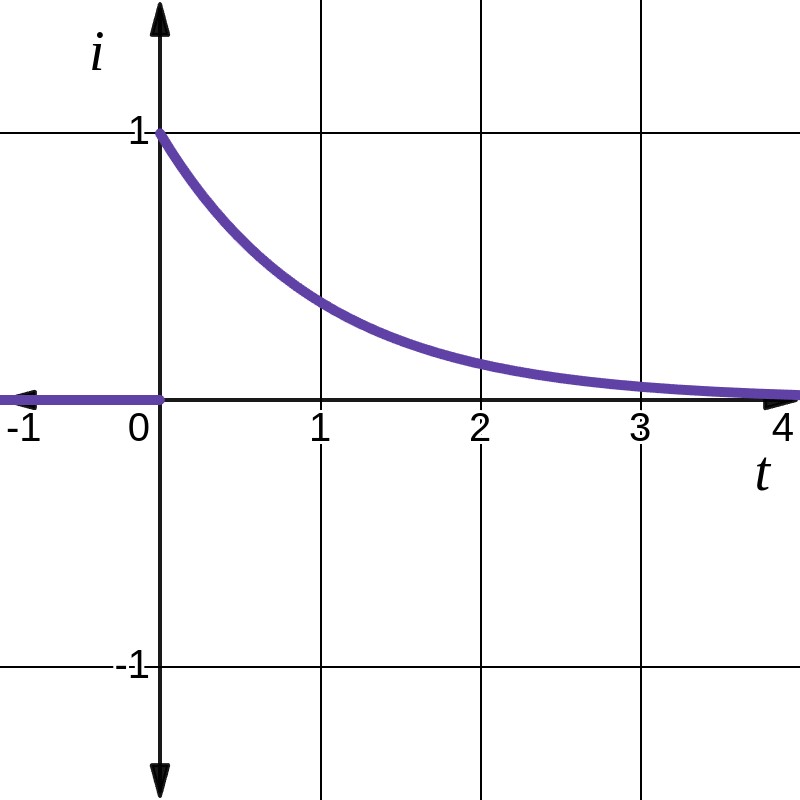
\includegraphics[width=1\textwidth]{./images/ej4.2.png}
          \textit{Respuesta a $u_t$}
        \end{minipage}
        \hspace{5mm}
        \begin{minipage}[h]{0.4\textwidth}
          \centering
          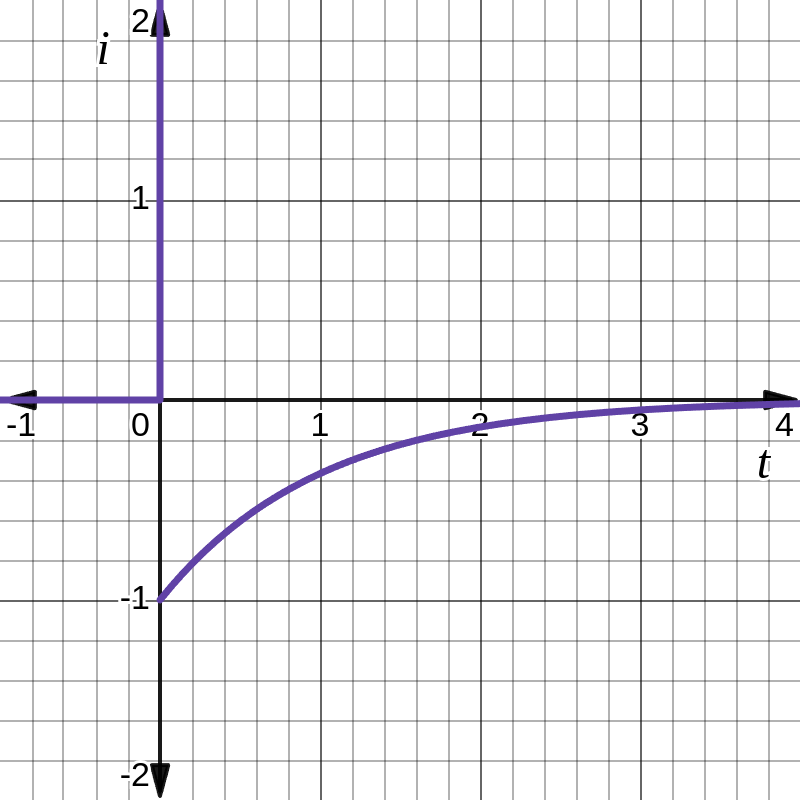
\includegraphics[width=1\textwidth]{./images/ej4.3.png}
          \textit{Respuesta a $\delta_t$}
        \end{minipage}
      \end{figure}

      Es importante mencionar cual es la razon de por la que el grafico de la respuesta al impulso es negativa.
      Esto se debe a que cuando el capacitor recibe el pico de corriente, se carga "instantaneamente"
      (el pico en $t=0$), y en el momento que deja de haber corriente circulando, el capacitor invierte el flujo de la
      misma, convirtiendose en "fuente" de corriente y voltaje.

      Una alternativa para poder llegar a calcular la respuesta del sistema por medio de la convolucion, es usar la
      propiedad de convolucion para la transformada de Laplace. Para ello, es necesario transformar la respuesta del
      sistema en $t$, a $s$:
      \begin{gather*}
        \mathbb{L}\left\{h(t)\right\} = \int_{0^-}^{\infty} \left(\frac{1}{R} \delta_t - \frac{1}{R^2C}e^{\frac{-t}{RC}} 
          \mu_t\right) \cdot e^{-st} dt\\
        ...\\
        \mathbb{L}\left\{h(t)\right\} = \frac{1}{R} - \frac{1}{R+R^2CS}\\
        \mathbb{L}\left\{h(t)\right\} = \frac{Cs}{1+RCs}
      \end{gather*}
      Como se puede ver, la transformada de laplace de la respuesta al impulso presenta un cero en $s = 0$, y solo
      presenta un polo en el eje real en $\left(-\frac{1}{RC},0\right)$:

      \noindent
      \begin{figure}[h]
        \centering
        \begin{minipage}[h]{0.4\textwidth}
          \centering
          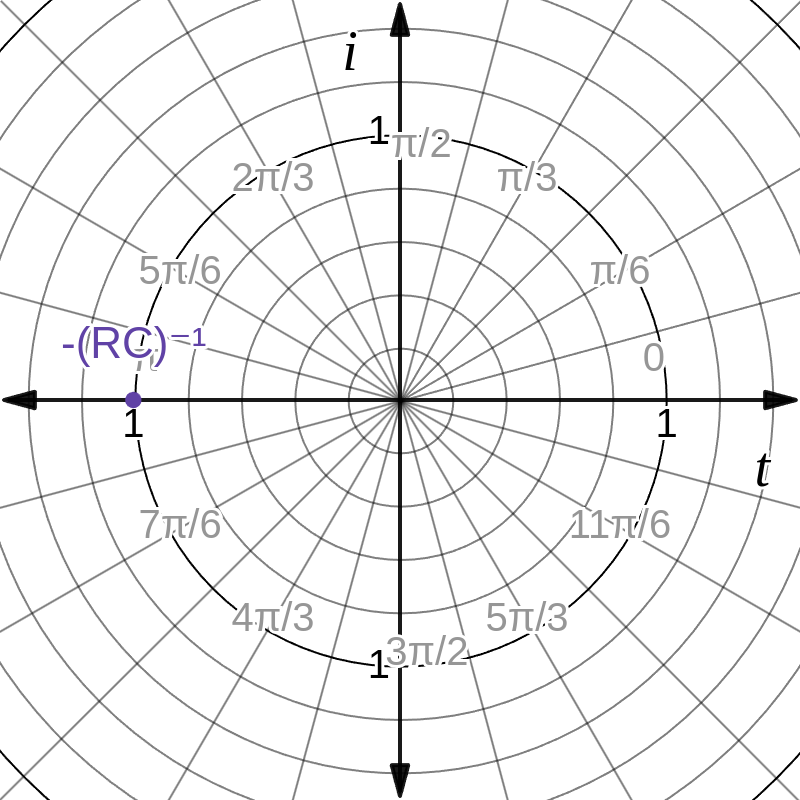
\includegraphics[width=1\textwidth]{./images/ej4.4.png}
          \textit{Polos de $H_s$}
        \end{minipage}
      \end{figure}

      Sabiendo el polo, ahora podemos decir con seguridad que la constante de tiempo del sistema, que es aquel $\tau$ 
      en el que el sistema alcanza el 63\% de su valor final, es:
      \begin{gather*}
        \tau = \frac{1}{|polo|} = \frac{1}{|-\frac{1}{RC}|} = RC
      \end{gather*}

      Ademas, ahora podemos tambien determinar los valores para $y(0)$ e $y(\infty)$ utilizando la transformada de
      Laplace, y los teoremas del valor inicial y valor final, que a groso modo, son hacer tender $sH(s)$ al
      infinito y a cero:
      \begin{align*}
        y(0^+) =& \lim_{s\to\infty} s \cdot \frac{Cs}{1+RCs} \hspace{3cm} &y(\infty) =& \lim_{s\to0} s \cdot
          \frac{Cs}{1+RCs}\\[6pt]
        y(0^+) =& \lim_{s\to\infty} \frac{Cs^2}{1+RCs} \hspace{3cm} &y(\infty) =& \lim_{s\to0} \frac{Cs^2}{1+RCs}\\[6pt]
        y(0^+) \to& \infty \hspace{3cm} &y(\infty) \to& 0
      \end{align*}
      Los valores obtenidos para el sistema tienen mucho sentido. Si le damos un analisis fisico, tiene sentido que
      cuando el circuito recibe el impulso, la corriente tiende a infinito, debido a que el capacitor "funciona" como
      un cortocircuito. Obviamente, en una situacion real, esto no se iria al infinito, si no que solamente tenderia a
      $\frac{V}{R}$, de tal forma que el capacitor actua como un cable.
      Asi mismo, cuando la funcion tiende al infinito, la corriente tiende a cero, debido a que ya el capacitor deberia
      estar completamente cargado, comportandose como un circuito abierto, y evitando la totalidad del paso de la
      corriente por el resto del circuito.

      Sabiendo que podemos aplicar la propiedad de transformada en el dominio del tiempo para Laplace, ahora podemos
      calcular la respuesta de otras funciones, como por ejemplo $h_t$, pero simplemente multiplicando $H_s$ y
      $\mathbb{L}\{\mu_t\}$:
      \begin{gather*}
        \mu_t * h_t \longleftrightarrow M_s \cdot H_s; \hspace{1cm}\mathbb{L}\{\mu_t\} = \frac{1}{s}\\[6pt]
        \mu_t * h_t \longleftrightarrow \frac{Cs}{1+RCs} \frac{1}{s}\\[6pt]
        \mu_t * h_t \longleftrightarrow \frac{Cs}{S+RCs^2}
      \end{gather*}


  \end{enumerate}

  \newpage
  \textbf{Circuito Eléctrico RLC:} circuito eléctrico correspondiente a un sistema de 2° orden y su ecuación
  caracteristica:
  \begin{equation*}
    v(t) = Ri_{(t)} + L \frac{d}{dt} i_{(t)} + \frac{1}{C} \int_{0}^{t} i_{(\tau)} d\tau
  \end{equation*}

  \vspace{-1cm}
  \noindent
  \begin{figure}[h]
    \centering
    \begin{minipage}[h]{0.5\textwidth}
      \centering
      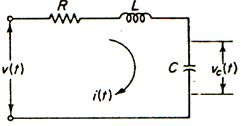
\includegraphics[width=1\textwidth]{./images/ej4.5.jpg}
      \textit{Circuito RLC}
    \end{minipage}
  \end{figure}

  \begin{enumerate}[label=\alph*)]
  \item Obtener una representación del circuito con Ecuaciones Diferenciales de segundo orden y coeficientes constantes,
    y con ello, definir un Sistema en tiempo continuo con entrada $x_{(t)} = v_{(t)}$ y salida $y_{(t)} = i_{(t)}$. Luego,
    hacer un diagrama de bloques de la E.D; exponiendo los integradores que la conforma.
    
    El circuito RLC esta descrito por la ecuacion caracteristica:
    \begin{equation*}
      v(t) = Ri_{(t)} + L \frac{d}{dt} i_{(t)} + \frac{1}{C} \int_{0}^{t} i_{(\tau)} d\tau
    \end{equation*}
    Para tener una nomenclatura mas generica, sustituimos la entrada $v(t)$ con $x(t)$ y la salida $i(t)$ con $y(t)$:
    \begin{equation*}
      x(t) = Ry_{(t)} + L \frac{d}{dt} y_{(t)} + \frac{1}{C} \int_{0}^{t} y_{(\tau)} d\tau
    \end{equation*}
    Teniendo en cuenta que $y(t)$ es la salida e $x(t)$ la entrada, las ecuaciones diferenciales toman la forma:
    \begin{equation*}
      \left(D^N + \sum_{i=0}^{N-1} a_i D^i\right) \cdot y(t) = \left(\sum_{i=0}^{M} b_i D^i\right) \cdot x(t)
    \end{equation*}
    Reacomodando la ecuacion caracteristica generalizada, nos queda:
    \begin{align*}
      D^1\left\{x_t\right\} &= D^1\left\{R y_t\right\} + D^2\left\{L y_t\right\} + \frac{1}{C} y_t\\
      D^1\left\{\frac{1}{L} x_t\right\} &= D^2\left\{y_t\right\} + D^1\left\{\frac{1}{RL} y_t\right\} + \frac{1}{LC} y_t\\
      \frac{dx_t}{dt} \frac{1}{L} &= \frac{d^2 y_t}{dt^2} + \frac{dy_t}{dt} \frac{1}{RL} + \frac{1}{LC} y_t
    \end{align*}
    Lo cual es la ecuacion diferencial de segundo orden a coeficientes constantes que describe el comportamiento
    del circuito RCL.

    Para el diagrama de simulacion solo tuvimos que integrar la ecuacion diferencial hasta que no hubo mas derivadores:
      
    \begin{figure}[h]
      \centering
      \begin{tikzpicture}[auto, node distance=2cm, >=Stealth, thick]
        % Definición de estilos para los bloques y sumador
        \tikzstyle{block} = [draw, rectangle, minimum height=1.5em, minimum width=3em]
        \tikzstyle{sum} = [draw, circle, inner sep=1pt, minimum size=1cm, node distance=2cm]
        \tikzstyle{connector} = [draw, fill, circle, minimum size=4pt, inner sep=0pt] % Estilo para el punto de conexión

         % Definición de nodos
        \node at (0,0) [coordinate] (input) {}; % Nodo de entrada
        \node [coordinate, on grid, right=7cm of input] (elbowInput1) {};
        \node [block, on grid, below=2cm of elbowInput1] (gainInput1) {$\frac{1}{C}$};
        \node [sum, on grid, below=2cm of gainInput1] (sum1) {$+$};
        \node [block, on grid, left=3cm of sum1] (integrator1) {$\int$};
        \node [block, on grid, right=3cm of sum1] (integrator2) {$\int$};
        \node [connector, on grid, left=3cm of integrator1] (elbowOutput1) {};
        \node [block, on grid, below=2cm of elbowOutput1] (gainOutput1) {$-\frac{1}{LC}$};
        \node [block, on grid, below=2cm of sum1] (gainOutput2) {$-\frac{R}{L}$};
        \node [coordinate, on grid, below=2cm of gainOutput1] (elbowOutput2) {};
        \node [connector, on grid, below=2cm of gainOutput2] (elbowOutput3) {};
        \node [coordinate, on grid, right=5cm of elbowOutput3] (elbowOutput4) {};
        \node [coordinate, on grid, above=4cm of elbowOutput4] (elbowOutput5) {};
        \node [coordinate, on grid, right=2cm of elbowOutput5] (output) {};

        % Conexiones entre nodos
        \draw [>-] (input) -- node {$x_t(t)$} (elbowInput1);
        \draw [->] (elbowInput1) -- (gainInput1);
        \draw [->] (gainInput1) -- (sum1);
        \draw [->] (elbowOutput1) -- (integrator1);
        \draw [->] (integrator1) -- (sum1);
        \draw [->] (sum1) -- (integrator2);
        \draw [-] (integrator2) -- (elbowOutput5);
        \draw [->] (elbowOutput5) -- node {$y_t(t)$} (output);
        \draw [-] (elbowOutput1) -- (gainOutput1);
        \draw [->] (elbowOutput2) -- (gainOutput1);
        \draw [-] (elbowOutput2) -- (elbowOutput3);
        \draw [-] (elbowOutput3) -- (elbowOutput4);
        \draw [->] (elbowOutput3) -- (gainOutput2);
        \draw [->] (gainOutput2) -- (sum1);
        \draw [-] (elbowOutput5) -- (elbowOutput4);
      \end{tikzpicture}
      \begin{equation*}
        y_t = D^{-2}\left\{-\frac{1}{RC} y_t\right\} + D^{-1}\left\{\frac{1}{C} x_t - \frac{R}{L}\right\}
      \end{equation*}
    \end{figure}


  \item Sea $y_t = S\{x_t\}$ el sistema obtenido de las soluciones al sistema de Ecuaciones Diferenciales del inciso
    anterior. Teniendo en cuenta el siguientes resultado matemático, obtener una descripción explicita de la respuesta
    transformada $Y_{(s)} = L\{y_t\} = L\{S\{x_t\}\}$:
  \begin{itemize}
    \item Sean $\alpha_1, \alpha_0, \beta_2, \beta_1, \beta_0 \in \mathbb{R}$ constantes; $y_{(t)}, x_{(t)}$ funciones
      con variable de tiempo continuo, las cuales verifican la ecuacion diferencial de segundo orden con coeficientes
      constantes:
      $$y_t^{''} + \alpha_1 y_t^{'} + \alpha_0 y_t = \beta_2 x_t^{''} + \beta_1 x_t^{'} + \beta_0 x_t$$
      Entonces, una Solucion General explicita de la Ecuacion Diferencial Transformada es:
      $$Y_{(s)} = \frac{\beta_2 s^2 + \beta_1 s + \beta_0}{s^2 + \alpha_1 s + \alpha_0}X_{(s)} + \frac{(y_0 - \beta_2 x_0)
        s + (\alpha_1 y_0 - \beta_1 x_0 + y_0^{'} - \beta_2 x_0^{'})}{s^2 + \alpha_1 s + \alpha_0}$$
      donde $Y_{(s)} = L\{y_t\}$, $X_{(s)} = L\{x_t\}$, con $s = \sigma + j \omega$ (variable compleja). Condiciones
      Iniciales arbitrarias; $y_0 = y(0), y_0^{'} = y^{'}(0), x_0 = x(0), x_0^{'} = x^{'}(0)$.
    \item Usando las propiedades de la transformada de Laplace, demostrar la igualdad propuesta para la funcion
     $Y_{(s)}$.
  \end{itemize}

  \item Restringir el sistema anterior a CI nulas y obtener la formula de la respuesta transformada $Y_{(s)} = L\{y\}$.
    Luego, calcular la Función de transferencia $H_{(s)} = L\{h_t\}$ donde $h_t$ es la respuesta al impulso del sistema
    linealizado. Luego, graficar en el plano complejo los polos y ceros de dicha función.

  \item Trabajar con el sistema linealizado del inciso anterior, y calcular la transformada
    $Y_1(s) = L\{S\{3\delta_{(t-2)}\}\}$, y similarmente $Y_2(s) = L\{S\{\mu_{(t+2)}\}\}$. Luego, implementar la técnica
    de anti-transformada para obtener las señales de respuesta en la variable de tiempo $y_1 = S\{3\delta_{(t-2)}\}$,
    $y_2 = S\{\mu_{(t+2)}\}$, respectivamente.\\
    \textbf{Reflexionar}: ¿En que variable están definidas las funciones $Y_1$, $Y_2$? ¿Que tipo de variable es $s$ y que
    diferencia tiene con la variable $t$? ¿Que diferencias se observan entres las funciones $Y_1$, $Y_2$ y sus señales
    $y_1$, $y_2$?

  \item Graficar en diagrama de bloques del sistema en el dominios de la variable compleja.  Determinar el coeficiente
    de amortiguamiento $\xi$ y la frecuencia natural $\omega_n$ del sistema linealizado.\\
    \textbf{Reflexionar}: ¿Que diferencias se observan entre el diagrama de bloques del inciso (a) y el diagrama de
    bloques del inciso (e)? ¿Las variables $s$ y $t$ están presentes de alguna forma en los diagramas mencionados? ¿Tiene
    algún significado subrayar que el diagrama esta en el dominio del tiempo o en el dominio complejo?

  \end{enumerate}
\end{document}
